\documentclass[twoside]{book}

% Packages required by doxygen
\usepackage{fixltx2e}
\usepackage{calc}
\usepackage{doxygen}
\usepackage[export]{adjustbox} % also loads graphicx
\usepackage{graphicx}
\usepackage[utf8]{inputenc}
\usepackage{makeidx}
\usepackage{multicol}
\usepackage{multirow}
\PassOptionsToPackage{warn}{textcomp}
\usepackage{textcomp}
\usepackage[nointegrals]{wasysym}
\usepackage[table]{xcolor}

% Font selection
\usepackage[T1]{fontenc}
\usepackage[scaled=.90]{helvet}
\usepackage{courier}
\usepackage{amssymb}
\usepackage{sectsty}
\renewcommand{\familydefault}{\sfdefault}
\allsectionsfont{%
  \fontseries{bc}\selectfont%
  \color{darkgray}%
}
\renewcommand{\DoxyLabelFont}{%
  \fontseries{bc}\selectfont%
  \color{darkgray}%
}
\newcommand{\+}{\discretionary{\mbox{\scriptsize$\hookleftarrow$}}{}{}}

% Page & text layout
\usepackage{geometry}
\geometry{%
  a4paper,%
  top=2.5cm,%
  bottom=2.5cm,%
  left=2.5cm,%
  right=2.5cm%
}
\tolerance=750
\hfuzz=15pt
\hbadness=750
\setlength{\emergencystretch}{15pt}
\setlength{\parindent}{0cm}
\setlength{\parskip}{3ex plus 2ex minus 2ex}
\makeatletter
\renewcommand{\paragraph}{%
  \@startsection{paragraph}{4}{0ex}{-1.0ex}{1.0ex}{%
    \normalfont\normalsize\bfseries\SS@parafont%
  }%
}
\renewcommand{\subparagraph}{%
  \@startsection{subparagraph}{5}{0ex}{-1.0ex}{1.0ex}{%
    \normalfont\normalsize\bfseries\SS@subparafont%
  }%
}
\makeatother

% Headers & footers
\usepackage{fancyhdr}
\pagestyle{fancyplain}
\fancyhead[LE]{\fancyplain{}{\bfseries\thepage}}
\fancyhead[CE]{\fancyplain{}{}}
\fancyhead[RE]{\fancyplain{}{\bfseries\leftmark}}
\fancyhead[LO]{\fancyplain{}{\bfseries\rightmark}}
\fancyhead[CO]{\fancyplain{}{}}
\fancyhead[RO]{\fancyplain{}{\bfseries\thepage}}
\fancyfoot[LE]{\fancyplain{}{}}
\fancyfoot[CE]{\fancyplain{}{}}
\fancyfoot[RE]{\fancyplain{}{\bfseries\scriptsize 制作者 Doxygen }}
\fancyfoot[LO]{\fancyplain{}{\bfseries\scriptsize 制作者 Doxygen }}
\fancyfoot[CO]{\fancyplain{}{}}
\fancyfoot[RO]{\fancyplain{}{}}
\renewcommand{\footrulewidth}{0.4pt}
\renewcommand{\chaptermark}[1]{%
  \markboth{#1}{}%
}
\renewcommand{\sectionmark}[1]{%
  \markright{\thesection\ #1}%
}

% Indices & bibliography
\usepackage{natbib}
\usepackage[titles]{tocloft}
\setcounter{tocdepth}{3}
\setcounter{secnumdepth}{5}
\makeindex

% Hyperlinks (required, but should be loaded last)
\usepackage{ifpdf}
\ifpdf
  \usepackage[pdftex,pagebackref=true]{hyperref}
\else
  \usepackage[ps2pdf,pagebackref=true]{hyperref}
\fi
\hypersetup{%
  colorlinks=true,%
  linkcolor=blue,%
  citecolor=blue,%
  unicode%
}

% Custom commands
\newcommand{\clearemptydoublepage}{%
  \newpage{\pagestyle{empty}\cleardoublepage}%
}

\usepackage{caption}
\captionsetup{labelsep=space,justification=centering,font={bf},singlelinecheck=off,skip=4pt,position=top}

%===== C O N T E N T S =====

\begin{document}

% Titlepage & ToC
\hypersetup{pageanchor=false,
             bookmarksnumbered=true,
             pdfencoding=unicode
            }
\pagenumbering{roman}
\begin{titlepage}
\vspace*{7cm}
\begin{center}%
{\Large Chess \\[1ex]\large 1.\+0 }\\
\vspace*{1cm}
{\large 制作者 Doxygen 1.8.11}\\
\end{center}
\end{titlepage}
\clearemptydoublepage
\tableofcontents
\clearemptydoublepage
\pagenumbering{arabic}
\hypersetup{pageanchor=true}

%--- Begin generated contents ---
\chapter{命名空间索引}
\section{命名空间列表}
这里列出了所有命名空间定义,附带简要说明\+:\begin{DoxyCompactList}
\item\contentsline{section}{\hyperlink{namespace_ui}{Ui} }{\pageref{dc/df0/namespace_ui}}{}
\end{DoxyCompactList}

\chapter{继承关系索引}
\section{类继承关系}
此继承关系列表按字典顺序粗略的排序\+: \begin{DoxyCompactList}
\item \contentsline{section}{chess\+Data}{\pageref{classchess_data}}{}
\item Q\+Dialog\begin{DoxyCompactList}
\item \contentsline{section}{guest\+Window}{\pageref{classguest_window}}{}
\item \contentsline{section}{host\+Window}{\pageref{classhost_window}}{}
\end{DoxyCompactList}
\item Q\+Main\+Window\begin{DoxyCompactList}
\item \contentsline{section}{Main\+Window}{\pageref{class_main_window}}{}
\end{DoxyCompactList}
\item Q\+Widget\begin{DoxyCompactList}
\item \contentsline{section}{chess\+Board}{\pageref{classchess_board}}{}
\end{DoxyCompactList}
\end{DoxyCompactList}

\chapter{类索引}
\section{类列表}
这里列出了所有类、结构、联合以及接口定义等,并附带简要说明\+:\begin{DoxyCompactList}
\item\contentsline{section}{\hyperlink{classchess_board}{chess\+Board} }{\pageref{d9/dbc/classchess_board}}{}
\item\contentsline{section}{\hyperlink{classchess_data}{chess\+Data} }{\pageref{d1/dd3/classchess_data}}{}
\item\contentsline{section}{\hyperlink{classguest_window}{guest\+Window} }{\pageref{df/dac/classguest_window}}{}
\item\contentsline{section}{\hyperlink{classhost_window}{host\+Window} }{\pageref{d2/d00/classhost_window}}{}
\item\contentsline{section}{\hyperlink{class_main_window}{Main\+Window} }{\pageref{d9/dc6/class_main_window}}{}
\end{DoxyCompactList}

\chapter{文件索引}
\section{文件列表}
这里列出了所有文件,并附带简要说明\+:\begin{DoxyCompactList}
\item\contentsline{section}{\hyperlink{chessboard_8h}{chessboard.\+h} }{\pageref{df/d3e/chessboard_8h}}{}
\item\contentsline{section}{\hyperlink{chessdata_8h}{chessdata.\+h} }{\pageref{da/dc8/chessdata_8h}}{}
\item\contentsline{section}{\hyperlink{guestwindow_8h}{guestwindow.\+h} }{\pageref{da/d92/guestwindow_8h}}{}
\item\contentsline{section}{\hyperlink{hostwindow_8h}{hostwindow.\+h} }{\pageref{d9/d90/hostwindow_8h}}{}
\item\contentsline{section}{\hyperlink{mainwindow_8h}{mainwindow.\+h} }{\pageref{d9/d53/mainwindow_8h}}{}
\end{DoxyCompactList}

\chapter{命名空间文档}
\hypertarget{namespace_ui}{}\section{Ui 命名空间参考}
\label{namespace_ui}\index{Ui@{Ui}}

\chapter{类说明}
\hypertarget{classchess_board}{}\section{chess\+Board类 参考}
\label{classchess_board}\index{chess\+Board@{chess\+Board}}


{\ttfamily \#include \char`\"{}chessboard.\+h\char`\"{}}



类 chess\+Board 继承关系图\+:
\nopagebreak
\begin{figure}[H]
\begin{center}
\leavevmode
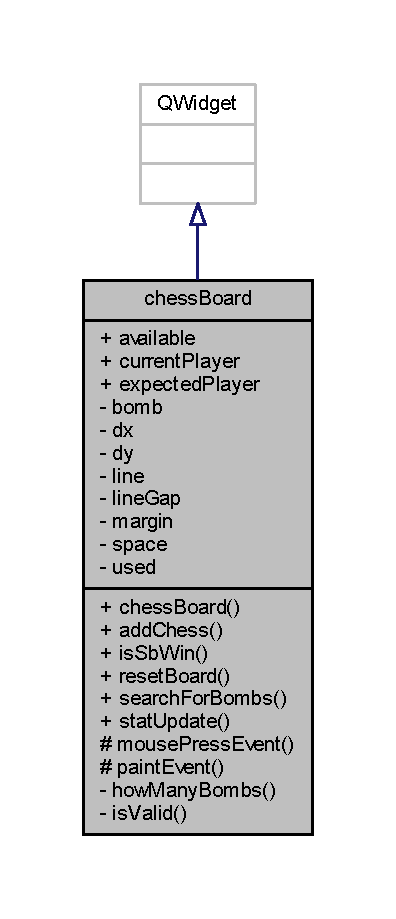
\includegraphics[width=190pt]{de/d0a/classchess_board__inherit__graph}
\end{center}
\end{figure}


chess\+Board 的协作图\+:
\nopagebreak
\begin{figure}[H]
\begin{center}
\leavevmode
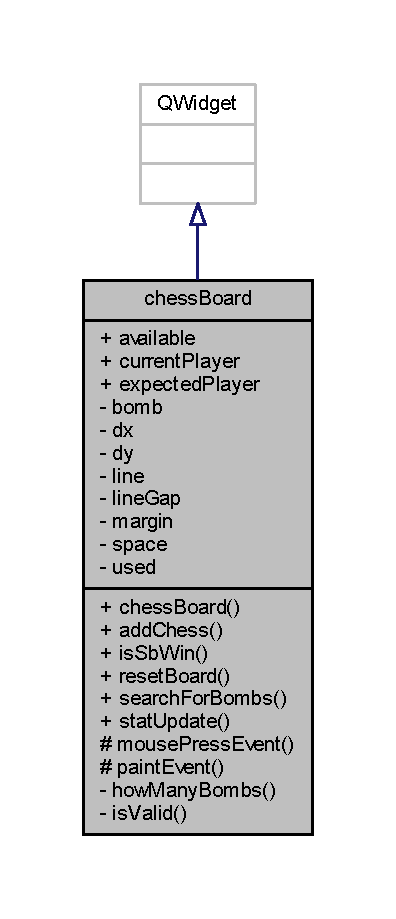
\includegraphics[width=190pt]{d5/db3/classchess_board__coll__graph}
\end{center}
\end{figure}
\subsection*{Public 槽}
\begin{DoxyCompactItemize}
\item 
void \hyperlink{classchess_board_a3a0e6a43b6ffd6f08a8a3b34fb5f9a5e_a3a0e6a43b6ffd6f08a8a3b34fb5f9a5e}{add\+Chess} (int x, int y)
\item 
int \hyperlink{classchess_board_a27433f6de7e03bdcb82a247a75e61ef2_a27433f6de7e03bdcb82a247a75e61ef2}{is\+Sb\+Win} ()
\item 
void \hyperlink{classchess_board_a685a53f93b9701359ba5d0bce447fef5_a685a53f93b9701359ba5d0bce447fef5}{reset\+Board} ()
\item 
void \hyperlink{classchess_board_aeed35797ed849bf9ac7527a0fb8e13a9_aeed35797ed849bf9ac7527a0fb8e13a9}{search\+For\+Bombs} ()
\item 
void \hyperlink{classchess_board_ac154f5bf7454a18b79a79af82aa700e5_ac154f5bf7454a18b79a79af82aa700e5}{stat\+Update} (int x, int y)
\end{DoxyCompactItemize}
\subsection*{信号}
\begin{DoxyCompactItemize}
\item 
void \hyperlink{classchess_board_ad33413fdd05cdedc6f63b56c3d0d5ced_ad33413fdd05cdedc6f63b56c3d0d5ced}{grid\+Clicked} (int, int)
\item 
void \hyperlink{classchess_board_ab05811b7fea74301f9169fe5e4e9b96f_ab05811b7fea74301f9169fe5e4e9b96f}{sb\+Win} (int)
\end{DoxyCompactItemize}
\subsection*{Public 成员函数}
\begin{DoxyCompactItemize}
\item 
\hyperlink{classchess_board_a3ffc09a4d95deaca0f6744ae25bb4f62_a3ffc09a4d95deaca0f6744ae25bb4f62}{chess\+Board} (Q\+Widget $\ast$parent=0)
\end{DoxyCompactItemize}
\subsection*{Public 属性}
\begin{DoxyCompactItemize}
\item 
bool \hyperlink{classchess_board_a7725e13857e6ddc2b155a9876ed4dea2_a7725e13857e6ddc2b155a9876ed4dea2}{available}
\item 
int \hyperlink{classchess_board_aedf4d34b20da347daf67987a1894062c_aedf4d34b20da347daf67987a1894062c}{current\+Player}
\item 
int \hyperlink{classchess_board_ade0d99898f63b66db3fa79d06c9bc350_ade0d99898f63b66db3fa79d06c9bc350}{expected\+Player}
\end{DoxyCompactItemize}
\subsection*{Protected 成员函数}
\begin{DoxyCompactItemize}
\item 
void \hyperlink{classchess_board_a234e4616abf11faa8dbc761eb21a6da7_a234e4616abf11faa8dbc761eb21a6da7}{mouse\+Press\+Event} (Q\+Mouse\+Event $\ast$ev)
\item 
void \hyperlink{classchess_board_aa7f58165ccd9b233e091e79b60c4bf38_aa7f58165ccd9b233e091e79b60c4bf38}{paint\+Event} (Q\+Paint\+Event $\ast$ev)
\end{DoxyCompactItemize}
\subsection*{Private 成员函数}
\begin{DoxyCompactItemize}
\item 
int \hyperlink{classchess_board_aa8c4b6997ffcdb121db319a1044f9658_aa8c4b6997ffcdb121db319a1044f9658}{how\+Many\+Bombs} ()
\item 
bool \hyperlink{classchess_board_ad0989442267fe68010ea2a289ec96344_ad0989442267fe68010ea2a289ec96344}{is\+Valid} (int x, int y)
\end{DoxyCompactItemize}
\subsection*{Private 属性}
\begin{DoxyCompactItemize}
\item 
bool \hyperlink{classchess_board_a6453bf0ce62eed140d37b294f3a4a8e8_a6453bf0ce62eed140d37b294f3a4a8e8}{bomb} \mbox{[}20\mbox{]}\mbox{[}20\mbox{]}
\item 
int \hyperlink{classchess_board_ac58f8fcb6344bb304616e95fd4773b5c_ac58f8fcb6344bb304616e95fd4773b5c}{dx} \mbox{[}8\mbox{]}
\item 
int \hyperlink{classchess_board_ac3fc44ec8c748e37f1e92dda4be8c03a_ac3fc44ec8c748e37f1e92dda4be8c03a}{dy} \mbox{[}8\mbox{]}
\item 
int \hyperlink{classchess_board_ad191786c9f76831e99699b315b24b1a5_ad191786c9f76831e99699b315b24b1a5}{line} \mbox{[}20\mbox{]}\mbox{[}20\mbox{]}\mbox{[}8\mbox{]}
\item 
int \hyperlink{classchess_board_aa871a25deb0dc97adcf79da0ce150467_aa871a25deb0dc97adcf79da0ce150467}{line\+Gap}
\item 
int \hyperlink{classchess_board_a86e2369dc84aac0e8c2ff5dfe395c9fa_a86e2369dc84aac0e8c2ff5dfe395c9fa}{margin}
\item 
int \hyperlink{classchess_board_a6ce69698dd39a950ccb031851296e9f7_a6ce69698dd39a950ccb031851296e9f7}{space} \mbox{[}20\mbox{]}\mbox{[}20\mbox{]}\mbox{[}8\mbox{]}
\item 
int \hyperlink{classchess_board_a606a859d2b32d470d04b0115ececc200_a606a859d2b32d470d04b0115ececc200}{used} \mbox{[}20\mbox{]}\mbox{[}20\mbox{]}
\end{DoxyCompactItemize}


\subsection{构造及析构函数说明}
\index{chess\+Board@{chess\+Board}!chess\+Board@{chess\+Board}}
\index{chess\+Board@{chess\+Board}!chess\+Board@{chess\+Board}}
\subsubsection[{\texorpdfstring{chess\+Board(\+Q\+Widget $\ast$parent=0)}{chessBoard(QWidget *parent=0)}}]{\setlength{\rightskip}{0pt plus 5cm}chess\+Board\+::chess\+Board (
\begin{DoxyParamCaption}
\item[{Q\+Widget $\ast$}]{parent = {\ttfamily 0}}
\end{DoxyParamCaption}
)\hspace{0.3cm}{\ttfamily [explicit]}}\hypertarget{classchess_board_a3ffc09a4d95deaca0f6744ae25bb4f62_a3ffc09a4d95deaca0f6744ae25bb4f62}{}\label{classchess_board_a3ffc09a4d95deaca0f6744ae25bb4f62_a3ffc09a4d95deaca0f6744ae25bb4f62}


\subsection{成员函数说明}
\index{chess\+Board@{chess\+Board}!add\+Chess@{add\+Chess}}
\index{add\+Chess@{add\+Chess}!chess\+Board@{chess\+Board}}
\subsubsection[{\texorpdfstring{add\+Chess}{addChess}}]{\setlength{\rightskip}{0pt plus 5cm}void chess\+Board\+::add\+Chess (
\begin{DoxyParamCaption}
\item[{int}]{x, }
\item[{int}]{y}
\end{DoxyParamCaption}
)\hspace{0.3cm}{\ttfamily [slot]}}\hypertarget{classchess_board_a3a0e6a43b6ffd6f08a8a3b34fb5f9a5e_a3a0e6a43b6ffd6f08a8a3b34fb5f9a5e}{}\label{classchess_board_a3a0e6a43b6ffd6f08a8a3b34fb5f9a5e_a3a0e6a43b6ffd6f08a8a3b34fb5f9a5e}
\index{chess\+Board@{chess\+Board}!grid\+Clicked@{grid\+Clicked}}
\index{grid\+Clicked@{grid\+Clicked}!chess\+Board@{chess\+Board}}
\subsubsection[{\texorpdfstring{grid\+Clicked}{gridClicked}}]{\setlength{\rightskip}{0pt plus 5cm}void chess\+Board\+::grid\+Clicked (
\begin{DoxyParamCaption}
\item[{int}]{, }
\item[{int}]{}
\end{DoxyParamCaption}
)\hspace{0.3cm}{\ttfamily [signal]}}\hypertarget{classchess_board_ad33413fdd05cdedc6f63b56c3d0d5ced_ad33413fdd05cdedc6f63b56c3d0d5ced}{}\label{classchess_board_ad33413fdd05cdedc6f63b56c3d0d5ced_ad33413fdd05cdedc6f63b56c3d0d5ced}
\index{chess\+Board@{chess\+Board}!how\+Many\+Bombs@{how\+Many\+Bombs}}
\index{how\+Many\+Bombs@{how\+Many\+Bombs}!chess\+Board@{chess\+Board}}
\subsubsection[{\texorpdfstring{how\+Many\+Bombs()}{howManyBombs()}}]{\setlength{\rightskip}{0pt plus 5cm}int chess\+Board\+::how\+Many\+Bombs (
\begin{DoxyParamCaption}
{}
\end{DoxyParamCaption}
)\hspace{0.3cm}{\ttfamily [private]}}\hypertarget{classchess_board_aa8c4b6997ffcdb121db319a1044f9658_aa8c4b6997ffcdb121db319a1044f9658}{}\label{classchess_board_aa8c4b6997ffcdb121db319a1044f9658_aa8c4b6997ffcdb121db319a1044f9658}
\index{chess\+Board@{chess\+Board}!is\+Sb\+Win@{is\+Sb\+Win}}
\index{is\+Sb\+Win@{is\+Sb\+Win}!chess\+Board@{chess\+Board}}
\subsubsection[{\texorpdfstring{is\+Sb\+Win}{isSbWin}}]{\setlength{\rightskip}{0pt plus 5cm}int chess\+Board\+::is\+Sb\+Win (
\begin{DoxyParamCaption}
{}
\end{DoxyParamCaption}
)\hspace{0.3cm}{\ttfamily [slot]}}\hypertarget{classchess_board_a27433f6de7e03bdcb82a247a75e61ef2_a27433f6de7e03bdcb82a247a75e61ef2}{}\label{classchess_board_a27433f6de7e03bdcb82a247a75e61ef2_a27433f6de7e03bdcb82a247a75e61ef2}
\index{chess\+Board@{chess\+Board}!is\+Valid@{is\+Valid}}
\index{is\+Valid@{is\+Valid}!chess\+Board@{chess\+Board}}
\subsubsection[{\texorpdfstring{is\+Valid(int x, int y)}{isValid(int x, int y)}}]{\setlength{\rightskip}{0pt plus 5cm}bool chess\+Board\+::is\+Valid (
\begin{DoxyParamCaption}
\item[{int}]{x, }
\item[{int}]{y}
\end{DoxyParamCaption}
)\hspace{0.3cm}{\ttfamily [private]}}\hypertarget{classchess_board_ad0989442267fe68010ea2a289ec96344_ad0989442267fe68010ea2a289ec96344}{}\label{classchess_board_ad0989442267fe68010ea2a289ec96344_ad0989442267fe68010ea2a289ec96344}
\index{chess\+Board@{chess\+Board}!mouse\+Press\+Event@{mouse\+Press\+Event}}
\index{mouse\+Press\+Event@{mouse\+Press\+Event}!chess\+Board@{chess\+Board}}
\subsubsection[{\texorpdfstring{mouse\+Press\+Event(\+Q\+Mouse\+Event $\ast$ev)}{mousePressEvent(QMouseEvent *ev)}}]{\setlength{\rightskip}{0pt plus 5cm}void chess\+Board\+::mouse\+Press\+Event (
\begin{DoxyParamCaption}
\item[{Q\+Mouse\+Event $\ast$}]{ev}
\end{DoxyParamCaption}
)\hspace{0.3cm}{\ttfamily [protected]}}\hypertarget{classchess_board_a234e4616abf11faa8dbc761eb21a6da7_a234e4616abf11faa8dbc761eb21a6da7}{}\label{classchess_board_a234e4616abf11faa8dbc761eb21a6da7_a234e4616abf11faa8dbc761eb21a6da7}
\index{chess\+Board@{chess\+Board}!paint\+Event@{paint\+Event}}
\index{paint\+Event@{paint\+Event}!chess\+Board@{chess\+Board}}
\subsubsection[{\texorpdfstring{paint\+Event(\+Q\+Paint\+Event $\ast$ev)}{paintEvent(QPaintEvent *ev)}}]{\setlength{\rightskip}{0pt plus 5cm}void chess\+Board\+::paint\+Event (
\begin{DoxyParamCaption}
\item[{Q\+Paint\+Event $\ast$}]{ev}
\end{DoxyParamCaption}
)\hspace{0.3cm}{\ttfamily [protected]}}\hypertarget{classchess_board_aa7f58165ccd9b233e091e79b60c4bf38_aa7f58165ccd9b233e091e79b60c4bf38}{}\label{classchess_board_aa7f58165ccd9b233e091e79b60c4bf38_aa7f58165ccd9b233e091e79b60c4bf38}
\index{chess\+Board@{chess\+Board}!reset\+Board@{reset\+Board}}
\index{reset\+Board@{reset\+Board}!chess\+Board@{chess\+Board}}
\subsubsection[{\texorpdfstring{reset\+Board}{resetBoard}}]{\setlength{\rightskip}{0pt plus 5cm}void chess\+Board\+::reset\+Board (
\begin{DoxyParamCaption}
{}
\end{DoxyParamCaption}
)\hspace{0.3cm}{\ttfamily [slot]}}\hypertarget{classchess_board_a685a53f93b9701359ba5d0bce447fef5_a685a53f93b9701359ba5d0bce447fef5}{}\label{classchess_board_a685a53f93b9701359ba5d0bce447fef5_a685a53f93b9701359ba5d0bce447fef5}
\index{chess\+Board@{chess\+Board}!sb\+Win@{sb\+Win}}
\index{sb\+Win@{sb\+Win}!chess\+Board@{chess\+Board}}
\subsubsection[{\texorpdfstring{sb\+Win}{sbWin}}]{\setlength{\rightskip}{0pt plus 5cm}void chess\+Board\+::sb\+Win (
\begin{DoxyParamCaption}
\item[{int}]{}
\end{DoxyParamCaption}
)\hspace{0.3cm}{\ttfamily [signal]}}\hypertarget{classchess_board_ab05811b7fea74301f9169fe5e4e9b96f_ab05811b7fea74301f9169fe5e4e9b96f}{}\label{classchess_board_ab05811b7fea74301f9169fe5e4e9b96f_ab05811b7fea74301f9169fe5e4e9b96f}
\index{chess\+Board@{chess\+Board}!search\+For\+Bombs@{search\+For\+Bombs}}
\index{search\+For\+Bombs@{search\+For\+Bombs}!chess\+Board@{chess\+Board}}
\subsubsection[{\texorpdfstring{search\+For\+Bombs}{searchForBombs}}]{\setlength{\rightskip}{0pt plus 5cm}void chess\+Board\+::search\+For\+Bombs (
\begin{DoxyParamCaption}
{}
\end{DoxyParamCaption}
)\hspace{0.3cm}{\ttfamily [slot]}}\hypertarget{classchess_board_aeed35797ed849bf9ac7527a0fb8e13a9_aeed35797ed849bf9ac7527a0fb8e13a9}{}\label{classchess_board_aeed35797ed849bf9ac7527a0fb8e13a9_aeed35797ed849bf9ac7527a0fb8e13a9}
\index{chess\+Board@{chess\+Board}!stat\+Update@{stat\+Update}}
\index{stat\+Update@{stat\+Update}!chess\+Board@{chess\+Board}}
\subsubsection[{\texorpdfstring{stat\+Update}{statUpdate}}]{\setlength{\rightskip}{0pt plus 5cm}void chess\+Board\+::stat\+Update (
\begin{DoxyParamCaption}
\item[{int}]{x, }
\item[{int}]{y}
\end{DoxyParamCaption}
)\hspace{0.3cm}{\ttfamily [slot]}}\hypertarget{classchess_board_ac154f5bf7454a18b79a79af82aa700e5_ac154f5bf7454a18b79a79af82aa700e5}{}\label{classchess_board_ac154f5bf7454a18b79a79af82aa700e5_ac154f5bf7454a18b79a79af82aa700e5}


\subsection{类成员变量说明}
\index{chess\+Board@{chess\+Board}!available@{available}}
\index{available@{available}!chess\+Board@{chess\+Board}}
\subsubsection[{\texorpdfstring{available}{available}}]{\setlength{\rightskip}{0pt plus 5cm}bool chess\+Board\+::available}\hypertarget{classchess_board_a7725e13857e6ddc2b155a9876ed4dea2_a7725e13857e6ddc2b155a9876ed4dea2}{}\label{classchess_board_a7725e13857e6ddc2b155a9876ed4dea2_a7725e13857e6ddc2b155a9876ed4dea2}
\index{chess\+Board@{chess\+Board}!bomb@{bomb}}
\index{bomb@{bomb}!chess\+Board@{chess\+Board}}
\subsubsection[{\texorpdfstring{bomb}{bomb}}]{\setlength{\rightskip}{0pt plus 5cm}bool chess\+Board\+::bomb\mbox{[}20\mbox{]}\mbox{[}20\mbox{]}\hspace{0.3cm}{\ttfamily [private]}}\hypertarget{classchess_board_a6453bf0ce62eed140d37b294f3a4a8e8_a6453bf0ce62eed140d37b294f3a4a8e8}{}\label{classchess_board_a6453bf0ce62eed140d37b294f3a4a8e8_a6453bf0ce62eed140d37b294f3a4a8e8}
\index{chess\+Board@{chess\+Board}!current\+Player@{current\+Player}}
\index{current\+Player@{current\+Player}!chess\+Board@{chess\+Board}}
\subsubsection[{\texorpdfstring{current\+Player}{currentPlayer}}]{\setlength{\rightskip}{0pt plus 5cm}int chess\+Board\+::current\+Player}\hypertarget{classchess_board_aedf4d34b20da347daf67987a1894062c_aedf4d34b20da347daf67987a1894062c}{}\label{classchess_board_aedf4d34b20da347daf67987a1894062c_aedf4d34b20da347daf67987a1894062c}
\index{chess\+Board@{chess\+Board}!dx@{dx}}
\index{dx@{dx}!chess\+Board@{chess\+Board}}
\subsubsection[{\texorpdfstring{dx}{dx}}]{\setlength{\rightskip}{0pt plus 5cm}int chess\+Board\+::dx\mbox{[}8\mbox{]}\hspace{0.3cm}{\ttfamily [private]}}\hypertarget{classchess_board_ac58f8fcb6344bb304616e95fd4773b5c_ac58f8fcb6344bb304616e95fd4773b5c}{}\label{classchess_board_ac58f8fcb6344bb304616e95fd4773b5c_ac58f8fcb6344bb304616e95fd4773b5c}
\index{chess\+Board@{chess\+Board}!dy@{dy}}
\index{dy@{dy}!chess\+Board@{chess\+Board}}
\subsubsection[{\texorpdfstring{dy}{dy}}]{\setlength{\rightskip}{0pt plus 5cm}int chess\+Board\+::dy\mbox{[}8\mbox{]}\hspace{0.3cm}{\ttfamily [private]}}\hypertarget{classchess_board_ac3fc44ec8c748e37f1e92dda4be8c03a_ac3fc44ec8c748e37f1e92dda4be8c03a}{}\label{classchess_board_ac3fc44ec8c748e37f1e92dda4be8c03a_ac3fc44ec8c748e37f1e92dda4be8c03a}
\index{chess\+Board@{chess\+Board}!expected\+Player@{expected\+Player}}
\index{expected\+Player@{expected\+Player}!chess\+Board@{chess\+Board}}
\subsubsection[{\texorpdfstring{expected\+Player}{expectedPlayer}}]{\setlength{\rightskip}{0pt plus 5cm}int chess\+Board\+::expected\+Player}\hypertarget{classchess_board_ade0d99898f63b66db3fa79d06c9bc350_ade0d99898f63b66db3fa79d06c9bc350}{}\label{classchess_board_ade0d99898f63b66db3fa79d06c9bc350_ade0d99898f63b66db3fa79d06c9bc350}
\index{chess\+Board@{chess\+Board}!line@{line}}
\index{line@{line}!chess\+Board@{chess\+Board}}
\subsubsection[{\texorpdfstring{line}{line}}]{\setlength{\rightskip}{0pt plus 5cm}int chess\+Board\+::line\mbox{[}20\mbox{]}\mbox{[}20\mbox{]}\mbox{[}8\mbox{]}\hspace{0.3cm}{\ttfamily [private]}}\hypertarget{classchess_board_ad191786c9f76831e99699b315b24b1a5_ad191786c9f76831e99699b315b24b1a5}{}\label{classchess_board_ad191786c9f76831e99699b315b24b1a5_ad191786c9f76831e99699b315b24b1a5}
\index{chess\+Board@{chess\+Board}!line\+Gap@{line\+Gap}}
\index{line\+Gap@{line\+Gap}!chess\+Board@{chess\+Board}}
\subsubsection[{\texorpdfstring{line\+Gap}{lineGap}}]{\setlength{\rightskip}{0pt plus 5cm}int chess\+Board\+::line\+Gap\hspace{0.3cm}{\ttfamily [private]}}\hypertarget{classchess_board_aa871a25deb0dc97adcf79da0ce150467_aa871a25deb0dc97adcf79da0ce150467}{}\label{classchess_board_aa871a25deb0dc97adcf79da0ce150467_aa871a25deb0dc97adcf79da0ce150467}
\index{chess\+Board@{chess\+Board}!margin@{margin}}
\index{margin@{margin}!chess\+Board@{chess\+Board}}
\subsubsection[{\texorpdfstring{margin}{margin}}]{\setlength{\rightskip}{0pt plus 5cm}int chess\+Board\+::margin\hspace{0.3cm}{\ttfamily [private]}}\hypertarget{classchess_board_a86e2369dc84aac0e8c2ff5dfe395c9fa_a86e2369dc84aac0e8c2ff5dfe395c9fa}{}\label{classchess_board_a86e2369dc84aac0e8c2ff5dfe395c9fa_a86e2369dc84aac0e8c2ff5dfe395c9fa}
\index{chess\+Board@{chess\+Board}!space@{space}}
\index{space@{space}!chess\+Board@{chess\+Board}}
\subsubsection[{\texorpdfstring{space}{space}}]{\setlength{\rightskip}{0pt plus 5cm}int chess\+Board\+::space\mbox{[}20\mbox{]}\mbox{[}20\mbox{]}\mbox{[}8\mbox{]}\hspace{0.3cm}{\ttfamily [private]}}\hypertarget{classchess_board_a6ce69698dd39a950ccb031851296e9f7_a6ce69698dd39a950ccb031851296e9f7}{}\label{classchess_board_a6ce69698dd39a950ccb031851296e9f7_a6ce69698dd39a950ccb031851296e9f7}
\index{chess\+Board@{chess\+Board}!used@{used}}
\index{used@{used}!chess\+Board@{chess\+Board}}
\subsubsection[{\texorpdfstring{used}{used}}]{\setlength{\rightskip}{0pt plus 5cm}int chess\+Board\+::used\mbox{[}20\mbox{]}\mbox{[}20\mbox{]}\hspace{0.3cm}{\ttfamily [private]}}\hypertarget{classchess_board_a606a859d2b32d470d04b0115ececc200_a606a859d2b32d470d04b0115ececc200}{}\label{classchess_board_a606a859d2b32d470d04b0115ececc200_a606a859d2b32d470d04b0115ececc200}


该类的文档由以下文件生成\+:\begin{DoxyCompactItemize}
\item 
\hyperlink{chessboard_8h}{chessboard.\+h}\end{DoxyCompactItemize}

\hypertarget{classchess_data}{}\section{chess\+Data类 参考}
\label{classchess_data}\index{chess\+Data@{chess\+Data}}


{\ttfamily \#include \char`\"{}chessdata.\+h\char`\"{}}



chess\+Data 的协作图\+:
\nopagebreak
\begin{figure}[H]
\begin{center}
\leavevmode
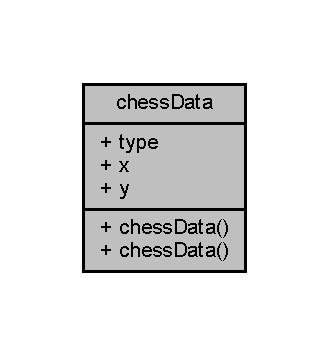
\includegraphics[width=158pt]{d5/df6/classchess_data__coll__graph}
\end{center}
\end{figure}
\subsection*{Public 成员函数}
\begin{DoxyCompactItemize}
\item 
\hyperlink{classchess_data_abd14890c77de3740cdd9a89c5d452c6d_abd14890c77de3740cdd9a89c5d452c6d}{chess\+Data} ()
\item 
\hyperlink{classchess_data_ad343300d63c53623de49c11b04765372_ad343300d63c53623de49c11b04765372}{chess\+Data} (int nx, int ny, int ntype)
\end{DoxyCompactItemize}
\subsection*{Public 属性}
\begin{DoxyCompactItemize}
\item 
int \hyperlink{classchess_data_ad67b369b475e8bcfc90c6da7f1210f0e_ad67b369b475e8bcfc90c6da7f1210f0e}{type}
\item 
int \hyperlink{classchess_data_aefa4c9a0412a6301112053d381f07f9d_aefa4c9a0412a6301112053d381f07f9d}{x}
\item 
int \hyperlink{classchess_data_ad9675434b53db8db40d423489e1aadac_ad9675434b53db8db40d423489e1aadac}{y}
\end{DoxyCompactItemize}


\subsection{构造及析构函数说明}
\index{chess\+Data@{chess\+Data}!chess\+Data@{chess\+Data}}
\index{chess\+Data@{chess\+Data}!chess\+Data@{chess\+Data}}
\subsubsection[{\texorpdfstring{chess\+Data()}{chessData()}}]{\setlength{\rightskip}{0pt plus 5cm}chess\+Data\+::chess\+Data (
\begin{DoxyParamCaption}
{}
\end{DoxyParamCaption}
)}\hypertarget{classchess_data_abd14890c77de3740cdd9a89c5d452c6d_abd14890c77de3740cdd9a89c5d452c6d}{}\label{classchess_data_abd14890c77de3740cdd9a89c5d452c6d_abd14890c77de3740cdd9a89c5d452c6d}
\index{chess\+Data@{chess\+Data}!chess\+Data@{chess\+Data}}
\index{chess\+Data@{chess\+Data}!chess\+Data@{chess\+Data}}
\subsubsection[{\texorpdfstring{chess\+Data(int nx, int ny, int ntype)}{chessData(int nx, int ny, int ntype)}}]{\setlength{\rightskip}{0pt plus 5cm}chess\+Data\+::chess\+Data (
\begin{DoxyParamCaption}
\item[{int}]{nx, }
\item[{int}]{ny, }
\item[{int}]{ntype}
\end{DoxyParamCaption}
)}\hypertarget{classchess_data_ad343300d63c53623de49c11b04765372_ad343300d63c53623de49c11b04765372}{}\label{classchess_data_ad343300d63c53623de49c11b04765372_ad343300d63c53623de49c11b04765372}


\subsection{类成员变量说明}
\index{chess\+Data@{chess\+Data}!type@{type}}
\index{type@{type}!chess\+Data@{chess\+Data}}
\subsubsection[{\texorpdfstring{type}{type}}]{\setlength{\rightskip}{0pt plus 5cm}int chess\+Data\+::type}\hypertarget{classchess_data_ad67b369b475e8bcfc90c6da7f1210f0e_ad67b369b475e8bcfc90c6da7f1210f0e}{}\label{classchess_data_ad67b369b475e8bcfc90c6da7f1210f0e_ad67b369b475e8bcfc90c6da7f1210f0e}
\index{chess\+Data@{chess\+Data}!x@{x}}
\index{x@{x}!chess\+Data@{chess\+Data}}
\subsubsection[{\texorpdfstring{x}{x}}]{\setlength{\rightskip}{0pt plus 5cm}int chess\+Data\+::x}\hypertarget{classchess_data_aefa4c9a0412a6301112053d381f07f9d_aefa4c9a0412a6301112053d381f07f9d}{}\label{classchess_data_aefa4c9a0412a6301112053d381f07f9d_aefa4c9a0412a6301112053d381f07f9d}
\index{chess\+Data@{chess\+Data}!y@{y}}
\index{y@{y}!chess\+Data@{chess\+Data}}
\subsubsection[{\texorpdfstring{y}{y}}]{\setlength{\rightskip}{0pt plus 5cm}int chess\+Data\+::y}\hypertarget{classchess_data_ad9675434b53db8db40d423489e1aadac_ad9675434b53db8db40d423489e1aadac}{}\label{classchess_data_ad9675434b53db8db40d423489e1aadac_ad9675434b53db8db40d423489e1aadac}


该类的文档由以下文件生成\+:\begin{DoxyCompactItemize}
\item 
\hyperlink{chessdata_8h}{chessdata.\+h}\end{DoxyCompactItemize}

\hypertarget{classguest_window}{}\section{guest\+Window类 参考}
\label{classguest_window}\index{guest\+Window@{guest\+Window}}


{\ttfamily \#include \char`\"{}guestwindow.\+h\char`\"{}}



类 guest\+Window 继承关系图\+:
\nopagebreak
\begin{figure}[H]
\begin{center}
\leavevmode
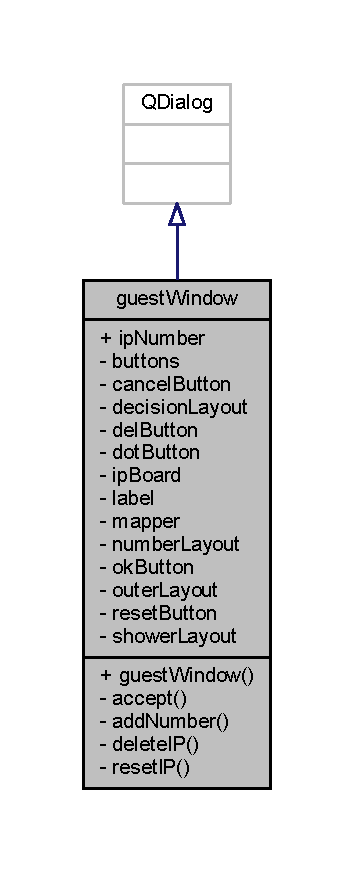
\includegraphics[width=170pt]{d5/dd1/classguest_window__inherit__graph}
\end{center}
\end{figure}


guest\+Window 的协作图\+:
\nopagebreak
\begin{figure}[H]
\begin{center}
\leavevmode
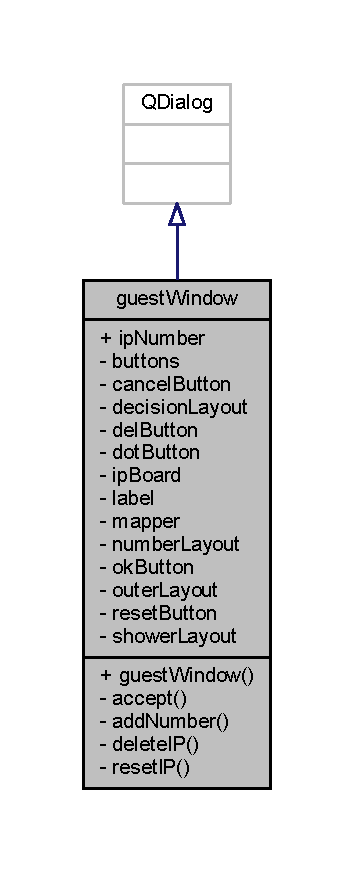
\includegraphics[width=170pt]{d8/d31/classguest_window__coll__graph}
\end{center}
\end{figure}
\subsection*{Public 成员函数}
\begin{DoxyCompactItemize}
\item 
\hyperlink{classguest_window_a969632c10abd2956bcc4187752b0a786_a969632c10abd2956bcc4187752b0a786}{guest\+Window} (Q\+Widget $\ast$parent=0)
\end{DoxyCompactItemize}
\subsection*{Public 属性}
\begin{DoxyCompactItemize}
\item 
Q\+String \hyperlink{classguest_window_aec5de0ba4a85a700539206dacb373722_aec5de0ba4a85a700539206dacb373722}{ip\+Number}
\end{DoxyCompactItemize}
\subsection*{Private 槽}
\begin{DoxyCompactItemize}
\item 
void \hyperlink{classguest_window_aac186524cb82d0776088d59ea84c5d54_aac186524cb82d0776088d59ea84c5d54}{accept} ()
\item 
void \hyperlink{classguest_window_a2400ccf7dd303656bfd6b66c212aa7ed_a2400ccf7dd303656bfd6b66c212aa7ed}{add\+Number} (int num)
\item 
void \hyperlink{classguest_window_a18c63e55961c253784e35e07f40d88ef_a18c63e55961c253784e35e07f40d88ef}{delete\+IP} ()
\item 
void \hyperlink{classguest_window_a51ef34507e3c18b981a9f0e62f36e9b4_a51ef34507e3c18b981a9f0e62f36e9b4}{reset\+IP} ()
\end{DoxyCompactItemize}
\subsection*{Private 属性}
\begin{DoxyCompactItemize}
\item 
Q\+Push\+Button $\ast$ \hyperlink{classguest_window_a9029a7872e4ba371605aa21a37c8c92c_a9029a7872e4ba371605aa21a37c8c92c}{buttons} \mbox{[}2\mbox{]}\mbox{[}5\mbox{]}
\item 
Q\+Push\+Button $\ast$ \hyperlink{classguest_window_ab9cf5b437951b3018d27e4f5189947e0_ab9cf5b437951b3018d27e4f5189947e0}{cancel\+Button}
\item 
Q\+Grid\+Layout $\ast$ \hyperlink{classguest_window_a1c4b57cfac6fe535b65cc8f4cc349d45_a1c4b57cfac6fe535b65cc8f4cc349d45}{decision\+Layout}
\item 
Q\+Push\+Button $\ast$ \hyperlink{classguest_window_a7a104c734623b3acabb007d6986921f3_a7a104c734623b3acabb007d6986921f3}{del\+Button}
\item 
Q\+Push\+Button $\ast$ \hyperlink{classguest_window_a681e5f9150088a9d3b83d5162155e564_a681e5f9150088a9d3b83d5162155e564}{dot\+Button}
\item 
Q\+Line\+Edit $\ast$ \hyperlink{classguest_window_aec27cc9e435045227442ee09bb099ba6_aec27cc9e435045227442ee09bb099ba6}{ip\+Board}
\item 
Q\+Label $\ast$ \hyperlink{classguest_window_aea635a4ae1aa3d18e24898fc2d36085a_aea635a4ae1aa3d18e24898fc2d36085a}{label}
\item 
Q\+Signal\+Mapper $\ast$ \hyperlink{classguest_window_a4dd35619381da82d6b3ff4debcd0e57b_a4dd35619381da82d6b3ff4debcd0e57b}{mapper}
\item 
Q\+Grid\+Layout $\ast$ \hyperlink{classguest_window_a103d25fd442d4efb826e91bc33533f87_a103d25fd442d4efb826e91bc33533f87}{number\+Layout}
\item 
Q\+Push\+Button $\ast$ \hyperlink{classguest_window_a324caba5a1eb67fc2f5f11d3b6adcdb2_a324caba5a1eb67fc2f5f11d3b6adcdb2}{ok\+Button}
\item 
Q\+V\+Box\+Layout $\ast$ \hyperlink{classguest_window_ab32add2cca7b39da8296afb5ce715064_ab32add2cca7b39da8296afb5ce715064}{outer\+Layout}
\item 
Q\+Push\+Button $\ast$ \hyperlink{classguest_window_a000c2ccdf75bdce1c46af14b61bffcd6_a000c2ccdf75bdce1c46af14b61bffcd6}{reset\+Button}
\item 
Q\+H\+Box\+Layout $\ast$ \hyperlink{classguest_window_aade794092a2f687a85c180b445260351_aade794092a2f687a85c180b445260351}{shower\+Layout}
\end{DoxyCompactItemize}


\subsection{构造及析构函数说明}
\index{guest\+Window@{guest\+Window}!guest\+Window@{guest\+Window}}
\index{guest\+Window@{guest\+Window}!guest\+Window@{guest\+Window}}
\subsubsection[{\texorpdfstring{guest\+Window(\+Q\+Widget $\ast$parent=0)}{guestWindow(QWidget *parent=0)}}]{\setlength{\rightskip}{0pt plus 5cm}guest\+Window\+::guest\+Window (
\begin{DoxyParamCaption}
\item[{Q\+Widget $\ast$}]{parent = {\ttfamily 0}}
\end{DoxyParamCaption}
)\hspace{0.3cm}{\ttfamily [explicit]}}\hypertarget{classguest_window_a969632c10abd2956bcc4187752b0a786_a969632c10abd2956bcc4187752b0a786}{}\label{classguest_window_a969632c10abd2956bcc4187752b0a786_a969632c10abd2956bcc4187752b0a786}


\subsection{成员函数说明}
\index{guest\+Window@{guest\+Window}!accept@{accept}}
\index{accept@{accept}!guest\+Window@{guest\+Window}}
\subsubsection[{\texorpdfstring{accept}{accept}}]{\setlength{\rightskip}{0pt plus 5cm}void guest\+Window\+::accept (
\begin{DoxyParamCaption}
{}
\end{DoxyParamCaption}
)\hspace{0.3cm}{\ttfamily [private]}, {\ttfamily [slot]}}\hypertarget{classguest_window_aac186524cb82d0776088d59ea84c5d54_aac186524cb82d0776088d59ea84c5d54}{}\label{classguest_window_aac186524cb82d0776088d59ea84c5d54_aac186524cb82d0776088d59ea84c5d54}
\index{guest\+Window@{guest\+Window}!add\+Number@{add\+Number}}
\index{add\+Number@{add\+Number}!guest\+Window@{guest\+Window}}
\subsubsection[{\texorpdfstring{add\+Number}{addNumber}}]{\setlength{\rightskip}{0pt plus 5cm}void guest\+Window\+::add\+Number (
\begin{DoxyParamCaption}
\item[{int}]{num}
\end{DoxyParamCaption}
)\hspace{0.3cm}{\ttfamily [private]}, {\ttfamily [slot]}}\hypertarget{classguest_window_a2400ccf7dd303656bfd6b66c212aa7ed_a2400ccf7dd303656bfd6b66c212aa7ed}{}\label{classguest_window_a2400ccf7dd303656bfd6b66c212aa7ed_a2400ccf7dd303656bfd6b66c212aa7ed}
\index{guest\+Window@{guest\+Window}!delete\+IP@{delete\+IP}}
\index{delete\+IP@{delete\+IP}!guest\+Window@{guest\+Window}}
\subsubsection[{\texorpdfstring{delete\+IP}{deleteIP}}]{\setlength{\rightskip}{0pt plus 5cm}void guest\+Window\+::delete\+IP (
\begin{DoxyParamCaption}
{}
\end{DoxyParamCaption}
)\hspace{0.3cm}{\ttfamily [private]}, {\ttfamily [slot]}}\hypertarget{classguest_window_a18c63e55961c253784e35e07f40d88ef_a18c63e55961c253784e35e07f40d88ef}{}\label{classguest_window_a18c63e55961c253784e35e07f40d88ef_a18c63e55961c253784e35e07f40d88ef}
\index{guest\+Window@{guest\+Window}!reset\+IP@{reset\+IP}}
\index{reset\+IP@{reset\+IP}!guest\+Window@{guest\+Window}}
\subsubsection[{\texorpdfstring{reset\+IP}{resetIP}}]{\setlength{\rightskip}{0pt plus 5cm}void guest\+Window\+::reset\+IP (
\begin{DoxyParamCaption}
{}
\end{DoxyParamCaption}
)\hspace{0.3cm}{\ttfamily [private]}, {\ttfamily [slot]}}\hypertarget{classguest_window_a51ef34507e3c18b981a9f0e62f36e9b4_a51ef34507e3c18b981a9f0e62f36e9b4}{}\label{classguest_window_a51ef34507e3c18b981a9f0e62f36e9b4_a51ef34507e3c18b981a9f0e62f36e9b4}


\subsection{类成员变量说明}
\index{guest\+Window@{guest\+Window}!buttons@{buttons}}
\index{buttons@{buttons}!guest\+Window@{guest\+Window}}
\subsubsection[{\texorpdfstring{buttons}{buttons}}]{\setlength{\rightskip}{0pt plus 5cm}Q\+Push\+Button$\ast$ guest\+Window\+::buttons\mbox{[}2\mbox{]}\mbox{[}5\mbox{]}\hspace{0.3cm}{\ttfamily [private]}}\hypertarget{classguest_window_a9029a7872e4ba371605aa21a37c8c92c_a9029a7872e4ba371605aa21a37c8c92c}{}\label{classguest_window_a9029a7872e4ba371605aa21a37c8c92c_a9029a7872e4ba371605aa21a37c8c92c}
\index{guest\+Window@{guest\+Window}!cancel\+Button@{cancel\+Button}}
\index{cancel\+Button@{cancel\+Button}!guest\+Window@{guest\+Window}}
\subsubsection[{\texorpdfstring{cancel\+Button}{cancelButton}}]{\setlength{\rightskip}{0pt plus 5cm}Q\+Push\+Button $\ast$ guest\+Window\+::cancel\+Button\hspace{0.3cm}{\ttfamily [private]}}\hypertarget{classguest_window_ab9cf5b437951b3018d27e4f5189947e0_ab9cf5b437951b3018d27e4f5189947e0}{}\label{classguest_window_ab9cf5b437951b3018d27e4f5189947e0_ab9cf5b437951b3018d27e4f5189947e0}
\index{guest\+Window@{guest\+Window}!decision\+Layout@{decision\+Layout}}
\index{decision\+Layout@{decision\+Layout}!guest\+Window@{guest\+Window}}
\subsubsection[{\texorpdfstring{decision\+Layout}{decisionLayout}}]{\setlength{\rightskip}{0pt plus 5cm}Q\+Grid\+Layout $\ast$ guest\+Window\+::decision\+Layout\hspace{0.3cm}{\ttfamily [private]}}\hypertarget{classguest_window_a1c4b57cfac6fe535b65cc8f4cc349d45_a1c4b57cfac6fe535b65cc8f4cc349d45}{}\label{classguest_window_a1c4b57cfac6fe535b65cc8f4cc349d45_a1c4b57cfac6fe535b65cc8f4cc349d45}
\index{guest\+Window@{guest\+Window}!del\+Button@{del\+Button}}
\index{del\+Button@{del\+Button}!guest\+Window@{guest\+Window}}
\subsubsection[{\texorpdfstring{del\+Button}{delButton}}]{\setlength{\rightskip}{0pt plus 5cm}Q\+Push\+Button $\ast$ guest\+Window\+::del\+Button\hspace{0.3cm}{\ttfamily [private]}}\hypertarget{classguest_window_a7a104c734623b3acabb007d6986921f3_a7a104c734623b3acabb007d6986921f3}{}\label{classguest_window_a7a104c734623b3acabb007d6986921f3_a7a104c734623b3acabb007d6986921f3}
\index{guest\+Window@{guest\+Window}!dot\+Button@{dot\+Button}}
\index{dot\+Button@{dot\+Button}!guest\+Window@{guest\+Window}}
\subsubsection[{\texorpdfstring{dot\+Button}{dotButton}}]{\setlength{\rightskip}{0pt plus 5cm}Q\+Push\+Button $\ast$ guest\+Window\+::dot\+Button\hspace{0.3cm}{\ttfamily [private]}}\hypertarget{classguest_window_a681e5f9150088a9d3b83d5162155e564_a681e5f9150088a9d3b83d5162155e564}{}\label{classguest_window_a681e5f9150088a9d3b83d5162155e564_a681e5f9150088a9d3b83d5162155e564}
\index{guest\+Window@{guest\+Window}!ip\+Board@{ip\+Board}}
\index{ip\+Board@{ip\+Board}!guest\+Window@{guest\+Window}}
\subsubsection[{\texorpdfstring{ip\+Board}{ipBoard}}]{\setlength{\rightskip}{0pt plus 5cm}Q\+Line\+Edit$\ast$ guest\+Window\+::ip\+Board\hspace{0.3cm}{\ttfamily [private]}}\hypertarget{classguest_window_aec27cc9e435045227442ee09bb099ba6_aec27cc9e435045227442ee09bb099ba6}{}\label{classguest_window_aec27cc9e435045227442ee09bb099ba6_aec27cc9e435045227442ee09bb099ba6}
\index{guest\+Window@{guest\+Window}!ip\+Number@{ip\+Number}}
\index{ip\+Number@{ip\+Number}!guest\+Window@{guest\+Window}}
\subsubsection[{\texorpdfstring{ip\+Number}{ipNumber}}]{\setlength{\rightskip}{0pt plus 5cm}Q\+String guest\+Window\+::ip\+Number}\hypertarget{classguest_window_aec5de0ba4a85a700539206dacb373722_aec5de0ba4a85a700539206dacb373722}{}\label{classguest_window_aec5de0ba4a85a700539206dacb373722_aec5de0ba4a85a700539206dacb373722}
\index{guest\+Window@{guest\+Window}!label@{label}}
\index{label@{label}!guest\+Window@{guest\+Window}}
\subsubsection[{\texorpdfstring{label}{label}}]{\setlength{\rightskip}{0pt plus 5cm}Q\+Label$\ast$ guest\+Window\+::label\hspace{0.3cm}{\ttfamily [private]}}\hypertarget{classguest_window_aea635a4ae1aa3d18e24898fc2d36085a_aea635a4ae1aa3d18e24898fc2d36085a}{}\label{classguest_window_aea635a4ae1aa3d18e24898fc2d36085a_aea635a4ae1aa3d18e24898fc2d36085a}
\index{guest\+Window@{guest\+Window}!mapper@{mapper}}
\index{mapper@{mapper}!guest\+Window@{guest\+Window}}
\subsubsection[{\texorpdfstring{mapper}{mapper}}]{\setlength{\rightskip}{0pt plus 5cm}Q\+Signal\+Mapper$\ast$ guest\+Window\+::mapper\hspace{0.3cm}{\ttfamily [private]}}\hypertarget{classguest_window_a4dd35619381da82d6b3ff4debcd0e57b_a4dd35619381da82d6b3ff4debcd0e57b}{}\label{classguest_window_a4dd35619381da82d6b3ff4debcd0e57b_a4dd35619381da82d6b3ff4debcd0e57b}
\index{guest\+Window@{guest\+Window}!number\+Layout@{number\+Layout}}
\index{number\+Layout@{number\+Layout}!guest\+Window@{guest\+Window}}
\subsubsection[{\texorpdfstring{number\+Layout}{numberLayout}}]{\setlength{\rightskip}{0pt plus 5cm}Q\+Grid\+Layout$\ast$ guest\+Window\+::number\+Layout\hspace{0.3cm}{\ttfamily [private]}}\hypertarget{classguest_window_a103d25fd442d4efb826e91bc33533f87_a103d25fd442d4efb826e91bc33533f87}{}\label{classguest_window_a103d25fd442d4efb826e91bc33533f87_a103d25fd442d4efb826e91bc33533f87}
\index{guest\+Window@{guest\+Window}!ok\+Button@{ok\+Button}}
\index{ok\+Button@{ok\+Button}!guest\+Window@{guest\+Window}}
\subsubsection[{\texorpdfstring{ok\+Button}{okButton}}]{\setlength{\rightskip}{0pt plus 5cm}Q\+Push\+Button $\ast$ guest\+Window\+::ok\+Button\hspace{0.3cm}{\ttfamily [private]}}\hypertarget{classguest_window_a324caba5a1eb67fc2f5f11d3b6adcdb2_a324caba5a1eb67fc2f5f11d3b6adcdb2}{}\label{classguest_window_a324caba5a1eb67fc2f5f11d3b6adcdb2_a324caba5a1eb67fc2f5f11d3b6adcdb2}
\index{guest\+Window@{guest\+Window}!outer\+Layout@{outer\+Layout}}
\index{outer\+Layout@{outer\+Layout}!guest\+Window@{guest\+Window}}
\subsubsection[{\texorpdfstring{outer\+Layout}{outerLayout}}]{\setlength{\rightskip}{0pt plus 5cm}Q\+V\+Box\+Layout$\ast$ guest\+Window\+::outer\+Layout\hspace{0.3cm}{\ttfamily [private]}}\hypertarget{classguest_window_ab32add2cca7b39da8296afb5ce715064_ab32add2cca7b39da8296afb5ce715064}{}\label{classguest_window_ab32add2cca7b39da8296afb5ce715064_ab32add2cca7b39da8296afb5ce715064}
\index{guest\+Window@{guest\+Window}!reset\+Button@{reset\+Button}}
\index{reset\+Button@{reset\+Button}!guest\+Window@{guest\+Window}}
\subsubsection[{\texorpdfstring{reset\+Button}{resetButton}}]{\setlength{\rightskip}{0pt plus 5cm}Q\+Push\+Button $\ast$ guest\+Window\+::reset\+Button\hspace{0.3cm}{\ttfamily [private]}}\hypertarget{classguest_window_a000c2ccdf75bdce1c46af14b61bffcd6_a000c2ccdf75bdce1c46af14b61bffcd6}{}\label{classguest_window_a000c2ccdf75bdce1c46af14b61bffcd6_a000c2ccdf75bdce1c46af14b61bffcd6}
\index{guest\+Window@{guest\+Window}!shower\+Layout@{shower\+Layout}}
\index{shower\+Layout@{shower\+Layout}!guest\+Window@{guest\+Window}}
\subsubsection[{\texorpdfstring{shower\+Layout}{showerLayout}}]{\setlength{\rightskip}{0pt plus 5cm}Q\+H\+Box\+Layout$\ast$ guest\+Window\+::shower\+Layout\hspace{0.3cm}{\ttfamily [private]}}\hypertarget{classguest_window_aade794092a2f687a85c180b445260351_aade794092a2f687a85c180b445260351}{}\label{classguest_window_aade794092a2f687a85c180b445260351_aade794092a2f687a85c180b445260351}


该类的文档由以下文件生成\+:\begin{DoxyCompactItemize}
\item 
\hyperlink{guestwindow_8h}{guestwindow.\+h}\end{DoxyCompactItemize}

\hypertarget{classhost_window}{}\section{host\+Window类 参考}
\label{classhost_window}\index{host\+Window@{host\+Window}}


{\ttfamily \#include \char`\"{}hostwindow.\+h\char`\"{}}



类 host\+Window 继承关系图\+:
\nopagebreak
\begin{figure}[H]
\begin{center}
\leavevmode
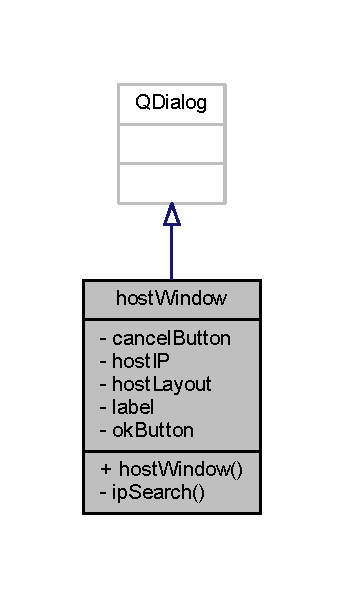
\includegraphics[width=165pt]{db/dc8/classhost_window__inherit__graph}
\end{center}
\end{figure}


host\+Window 的协作图\+:
\nopagebreak
\begin{figure}[H]
\begin{center}
\leavevmode
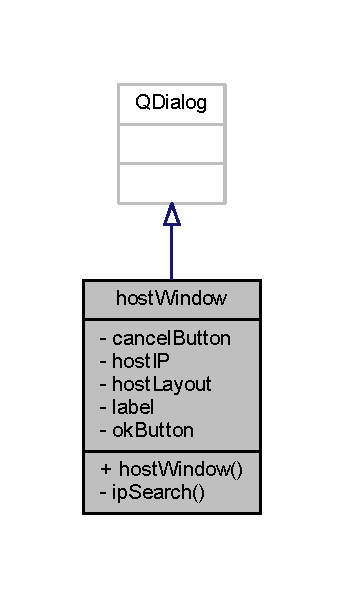
\includegraphics[width=165pt]{df/d46/classhost_window__coll__graph}
\end{center}
\end{figure}
\subsection*{Public 成员函数}
\begin{DoxyCompactItemize}
\item 
\hyperlink{classhost_window_acfe961f36b766fc3a1140b6e633d3925_acfe961f36b766fc3a1140b6e633d3925}{host\+Window} (Q\+Widget $\ast$parent=0)
\end{DoxyCompactItemize}
\subsection*{Private 成员函数}
\begin{DoxyCompactItemize}
\item 
Q\+String \hyperlink{classhost_window_aabfa278b993368b59aa65311b256926a_aabfa278b993368b59aa65311b256926a}{ip\+Search} ()
\end{DoxyCompactItemize}
\subsection*{Private 属性}
\begin{DoxyCompactItemize}
\item 
Q\+Push\+Button $\ast$ \hyperlink{classhost_window_a8fe146290eaba177d1f14d207725ea76_a8fe146290eaba177d1f14d207725ea76}{cancel\+Button}
\item 
Q\+Line\+Edit $\ast$ \hyperlink{classhost_window_aa5e9ae69f635b0a98c5b588b67f66641_aa5e9ae69f635b0a98c5b588b67f66641}{host\+IP}
\item 
Q\+Grid\+Layout $\ast$ \hyperlink{classhost_window_a030a018c2a4e6bc7af999828a0934ef8_a030a018c2a4e6bc7af999828a0934ef8}{host\+Layout}
\item 
Q\+Label $\ast$ \hyperlink{classhost_window_a59f675f1d69728ab3d87c814bf04eb83_a59f675f1d69728ab3d87c814bf04eb83}{label}
\item 
Q\+Push\+Button $\ast$ \hyperlink{classhost_window_aae2ab50869ebb07d4085fbc88d1fb0de_aae2ab50869ebb07d4085fbc88d1fb0de}{ok\+Button}
\end{DoxyCompactItemize}


\subsection{构造及析构函数说明}
\index{host\+Window@{host\+Window}!host\+Window@{host\+Window}}
\index{host\+Window@{host\+Window}!host\+Window@{host\+Window}}
\subsubsection[{\texorpdfstring{host\+Window(\+Q\+Widget $\ast$parent=0)}{hostWindow(QWidget *parent=0)}}]{\setlength{\rightskip}{0pt plus 5cm}host\+Window\+::host\+Window (
\begin{DoxyParamCaption}
\item[{Q\+Widget $\ast$}]{parent = {\ttfamily 0}}
\end{DoxyParamCaption}
)\hspace{0.3cm}{\ttfamily [explicit]}}\hypertarget{classhost_window_acfe961f36b766fc3a1140b6e633d3925_acfe961f36b766fc3a1140b6e633d3925}{}\label{classhost_window_acfe961f36b766fc3a1140b6e633d3925_acfe961f36b766fc3a1140b6e633d3925}


\subsection{成员函数说明}
\index{host\+Window@{host\+Window}!ip\+Search@{ip\+Search}}
\index{ip\+Search@{ip\+Search}!host\+Window@{host\+Window}}
\subsubsection[{\texorpdfstring{ip\+Search()}{ipSearch()}}]{\setlength{\rightskip}{0pt plus 5cm}Q\+String host\+Window\+::ip\+Search (
\begin{DoxyParamCaption}
{}
\end{DoxyParamCaption}
)\hspace{0.3cm}{\ttfamily [private]}}\hypertarget{classhost_window_aabfa278b993368b59aa65311b256926a_aabfa278b993368b59aa65311b256926a}{}\label{classhost_window_aabfa278b993368b59aa65311b256926a_aabfa278b993368b59aa65311b256926a}


\subsection{类成员变量说明}
\index{host\+Window@{host\+Window}!cancel\+Button@{cancel\+Button}}
\index{cancel\+Button@{cancel\+Button}!host\+Window@{host\+Window}}
\subsubsection[{\texorpdfstring{cancel\+Button}{cancelButton}}]{\setlength{\rightskip}{0pt plus 5cm}Q\+Push\+Button $\ast$ host\+Window\+::cancel\+Button\hspace{0.3cm}{\ttfamily [private]}}\hypertarget{classhost_window_a8fe146290eaba177d1f14d207725ea76_a8fe146290eaba177d1f14d207725ea76}{}\label{classhost_window_a8fe146290eaba177d1f14d207725ea76_a8fe146290eaba177d1f14d207725ea76}
\index{host\+Window@{host\+Window}!host\+IP@{host\+IP}}
\index{host\+IP@{host\+IP}!host\+Window@{host\+Window}}
\subsubsection[{\texorpdfstring{host\+IP}{hostIP}}]{\setlength{\rightskip}{0pt plus 5cm}Q\+Line\+Edit$\ast$ host\+Window\+::host\+IP\hspace{0.3cm}{\ttfamily [private]}}\hypertarget{classhost_window_aa5e9ae69f635b0a98c5b588b67f66641_aa5e9ae69f635b0a98c5b588b67f66641}{}\label{classhost_window_aa5e9ae69f635b0a98c5b588b67f66641_aa5e9ae69f635b0a98c5b588b67f66641}
\index{host\+Window@{host\+Window}!host\+Layout@{host\+Layout}}
\index{host\+Layout@{host\+Layout}!host\+Window@{host\+Window}}
\subsubsection[{\texorpdfstring{host\+Layout}{hostLayout}}]{\setlength{\rightskip}{0pt plus 5cm}Q\+Grid\+Layout$\ast$ host\+Window\+::host\+Layout\hspace{0.3cm}{\ttfamily [private]}}\hypertarget{classhost_window_a030a018c2a4e6bc7af999828a0934ef8_a030a018c2a4e6bc7af999828a0934ef8}{}\label{classhost_window_a030a018c2a4e6bc7af999828a0934ef8_a030a018c2a4e6bc7af999828a0934ef8}
\index{host\+Window@{host\+Window}!label@{label}}
\index{label@{label}!host\+Window@{host\+Window}}
\subsubsection[{\texorpdfstring{label}{label}}]{\setlength{\rightskip}{0pt plus 5cm}Q\+Label$\ast$ host\+Window\+::label\hspace{0.3cm}{\ttfamily [private]}}\hypertarget{classhost_window_a59f675f1d69728ab3d87c814bf04eb83_a59f675f1d69728ab3d87c814bf04eb83}{}\label{classhost_window_a59f675f1d69728ab3d87c814bf04eb83_a59f675f1d69728ab3d87c814bf04eb83}
\index{host\+Window@{host\+Window}!ok\+Button@{ok\+Button}}
\index{ok\+Button@{ok\+Button}!host\+Window@{host\+Window}}
\subsubsection[{\texorpdfstring{ok\+Button}{okButton}}]{\setlength{\rightskip}{0pt plus 5cm}Q\+Push\+Button$\ast$ host\+Window\+::ok\+Button\hspace{0.3cm}{\ttfamily [private]}}\hypertarget{classhost_window_aae2ab50869ebb07d4085fbc88d1fb0de_aae2ab50869ebb07d4085fbc88d1fb0de}{}\label{classhost_window_aae2ab50869ebb07d4085fbc88d1fb0de_aae2ab50869ebb07d4085fbc88d1fb0de}


该类的文档由以下文件生成\+:\begin{DoxyCompactItemize}
\item 
\hyperlink{hostwindow_8h}{hostwindow.\+h}\end{DoxyCompactItemize}

\hypertarget{class_main_window}{}\section{Main\+Window类 参考}
\label{class_main_window}\index{Main\+Window@{Main\+Window}}


{\ttfamily \#include \char`\"{}mainwindow.\+h\char`\"{}}



类 Main\+Window 继承关系图\+:
\nopagebreak
\begin{figure}[H]
\begin{center}
\leavevmode
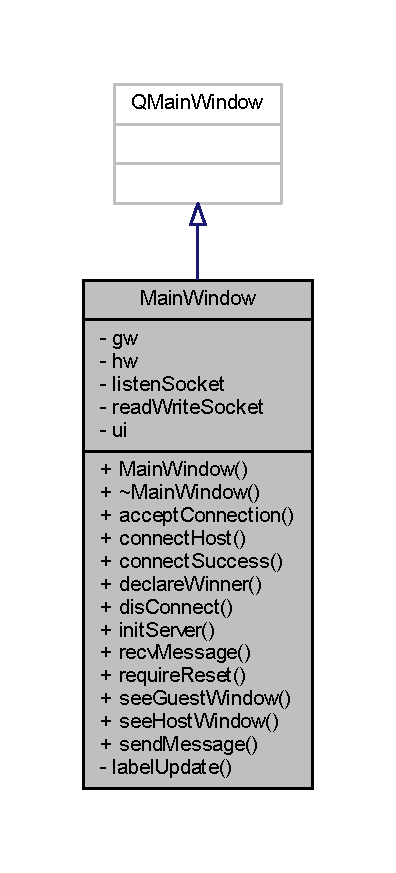
\includegraphics[width=190pt]{de/d4b/class_main_window__inherit__graph}
\end{center}
\end{figure}


Main\+Window 的协作图\+:
\nopagebreak
\begin{figure}[H]
\begin{center}
\leavevmode
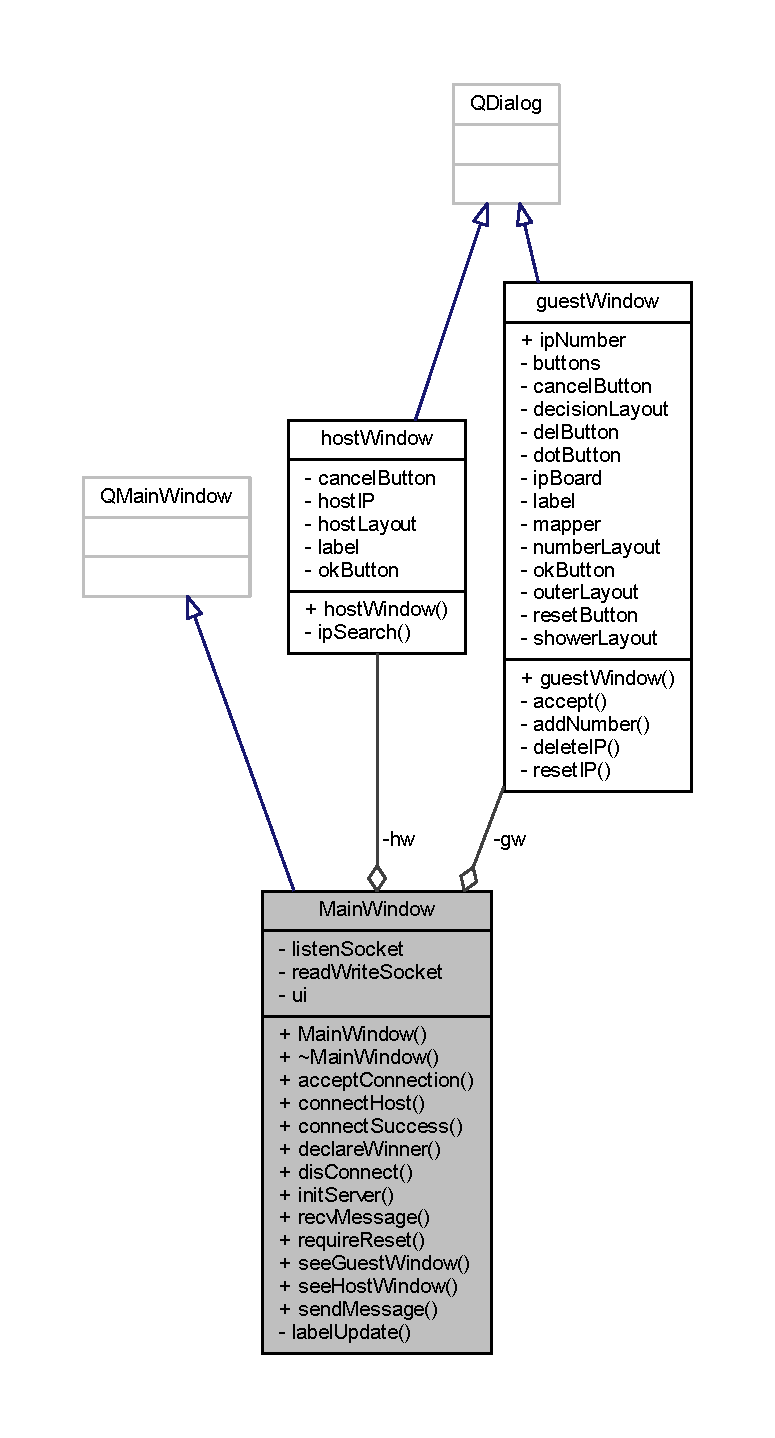
\includegraphics[height=550pt]{d0/db8/class_main_window__coll__graph}
\end{center}
\end{figure}
\subsection*{Public 槽}
\begin{DoxyCompactItemize}
\item 
void \hyperlink{class_main_window_ac24d6fd52a86d2f51570b4533faa5785_ac24d6fd52a86d2f51570b4533faa5785}{accept\+Connection} ()
\item 
void \hyperlink{class_main_window_a34b9342e6faff00c7d5c4c1ddfde6758_a34b9342e6faff00c7d5c4c1ddfde6758}{connect\+Host} (Q\+String add)
\item 
void \hyperlink{class_main_window_a818e9bdc274af691c4ebdbd255ede285_a818e9bdc274af691c4ebdbd255ede285}{connect\+Success} ()
\item 
void \hyperlink{class_main_window_abc7cfc8fb5680e5b2447d903174590ae_abc7cfc8fb5680e5b2447d903174590ae}{declare\+Winner} (int t)
\item 
void \hyperlink{class_main_window_a7ea49bac0b7604a1a4ba0dabb79b3439_a7ea49bac0b7604a1a4ba0dabb79b3439}{dis\+Connect} ()
\item 
void \hyperlink{class_main_window_a9343e215240dbbabcc2a9f83b1a53807_a9343e215240dbbabcc2a9f83b1a53807}{init\+Server} ()
\item 
void \hyperlink{class_main_window_a76637688e60dce665f72f661e1894412_a76637688e60dce665f72f661e1894412}{recv\+Message} ()
\item 
void \hyperlink{class_main_window_a939d1ea323f91e4a6e56e72ea3439803_a939d1ea323f91e4a6e56e72ea3439803}{require\+Reset} ()
\item 
void \hyperlink{class_main_window_a0b946fa967217fdf44022c00294f03b8_a0b946fa967217fdf44022c00294f03b8}{see\+Guest\+Window} ()
\item 
void \hyperlink{class_main_window_af89f09b9a2c59e4903d26b2bd1355052_af89f09b9a2c59e4903d26b2bd1355052}{see\+Host\+Window} ()
\item 
void \hyperlink{class_main_window_a6a0abf778996f6f2e3dc0d835d5f66ca_a6a0abf778996f6f2e3dc0d835d5f66ca}{send\+Message} (int i, int j)
\end{DoxyCompactItemize}
\subsection*{Public 成员函数}
\begin{DoxyCompactItemize}
\item 
\hyperlink{class_main_window_a8b244be8b7b7db1b08de2a2acb9409db_a8b244be8b7b7db1b08de2a2acb9409db}{Main\+Window} (Q\+Widget $\ast$parent=0)
\item 
\hyperlink{class_main_window_ae98d00a93bc118200eeef9f9bba1dba7_ae98d00a93bc118200eeef9f9bba1dba7}{$\sim$\+Main\+Window} ()
\end{DoxyCompactItemize}
\subsection*{Private 成员函数}
\begin{DoxyCompactItemize}
\item 
void \hyperlink{class_main_window_a09e3a622889962737a7f842b4f2a9693_a09e3a622889962737a7f842b4f2a9693}{label\+Update} ()
\end{DoxyCompactItemize}
\subsection*{Private 属性}
\begin{DoxyCompactItemize}
\item 
\hyperlink{classguest_window}{guest\+Window} $\ast$ \hyperlink{class_main_window_a2ff9360aec66a22cda39d9b9b12b1a48_a2ff9360aec66a22cda39d9b9b12b1a48}{gw}
\item 
\hyperlink{classhost_window}{host\+Window} $\ast$ \hyperlink{class_main_window_a4bd514a5ac9fb14a666d3e056f7d48ef_a4bd514a5ac9fb14a666d3e056f7d48ef}{hw}
\item 
Q\+Tcp\+Server $\ast$ \hyperlink{class_main_window_a15e38a8a7fc8737287a4a182bc824534_a15e38a8a7fc8737287a4a182bc824534}{listen\+Socket}
\item 
Q\+Tcp\+Socket $\ast$ \hyperlink{class_main_window_a5189009165424634032c2f04a1dc46fe_a5189009165424634032c2f04a1dc46fe}{read\+Write\+Socket}
\item 
Ui\+::\+Main\+Window $\ast$ \hyperlink{class_main_window_a35466a70ed47252a0191168126a352a5_a35466a70ed47252a0191168126a352a5}{ui}
\end{DoxyCompactItemize}


\subsection{构造及析构函数说明}
\index{Main\+Window@{Main\+Window}!Main\+Window@{Main\+Window}}
\index{Main\+Window@{Main\+Window}!Main\+Window@{Main\+Window}}
\subsubsection[{\texorpdfstring{Main\+Window(\+Q\+Widget $\ast$parent=0)}{MainWindow(QWidget *parent=0)}}]{\setlength{\rightskip}{0pt plus 5cm}Main\+Window\+::\+Main\+Window (
\begin{DoxyParamCaption}
\item[{Q\+Widget $\ast$}]{parent = {\ttfamily 0}}
\end{DoxyParamCaption}
)\hspace{0.3cm}{\ttfamily [explicit]}}\hypertarget{class_main_window_a8b244be8b7b7db1b08de2a2acb9409db_a8b244be8b7b7db1b08de2a2acb9409db}{}\label{class_main_window_a8b244be8b7b7db1b08de2a2acb9409db_a8b244be8b7b7db1b08de2a2acb9409db}
\index{Main\+Window@{Main\+Window}!````~Main\+Window@{$\sim$\+Main\+Window}}
\index{````~Main\+Window@{$\sim$\+Main\+Window}!Main\+Window@{Main\+Window}}
\subsubsection[{\texorpdfstring{$\sim$\+Main\+Window()}{~MainWindow()}}]{\setlength{\rightskip}{0pt plus 5cm}Main\+Window\+::$\sim$\+Main\+Window (
\begin{DoxyParamCaption}
{}
\end{DoxyParamCaption}
)}\hypertarget{class_main_window_ae98d00a93bc118200eeef9f9bba1dba7_ae98d00a93bc118200eeef9f9bba1dba7}{}\label{class_main_window_ae98d00a93bc118200eeef9f9bba1dba7_ae98d00a93bc118200eeef9f9bba1dba7}


\subsection{成员函数说明}
\index{Main\+Window@{Main\+Window}!accept\+Connection@{accept\+Connection}}
\index{accept\+Connection@{accept\+Connection}!Main\+Window@{Main\+Window}}
\subsubsection[{\texorpdfstring{accept\+Connection}{acceptConnection}}]{\setlength{\rightskip}{0pt plus 5cm}void Main\+Window\+::accept\+Connection (
\begin{DoxyParamCaption}
{}
\end{DoxyParamCaption}
)\hspace{0.3cm}{\ttfamily [slot]}}\hypertarget{class_main_window_ac24d6fd52a86d2f51570b4533faa5785_ac24d6fd52a86d2f51570b4533faa5785}{}\label{class_main_window_ac24d6fd52a86d2f51570b4533faa5785_ac24d6fd52a86d2f51570b4533faa5785}
\index{Main\+Window@{Main\+Window}!connect\+Host@{connect\+Host}}
\index{connect\+Host@{connect\+Host}!Main\+Window@{Main\+Window}}
\subsubsection[{\texorpdfstring{connect\+Host}{connectHost}}]{\setlength{\rightskip}{0pt plus 5cm}void Main\+Window\+::connect\+Host (
\begin{DoxyParamCaption}
\item[{Q\+String}]{add}
\end{DoxyParamCaption}
)\hspace{0.3cm}{\ttfamily [slot]}}\hypertarget{class_main_window_a34b9342e6faff00c7d5c4c1ddfde6758_a34b9342e6faff00c7d5c4c1ddfde6758}{}\label{class_main_window_a34b9342e6faff00c7d5c4c1ddfde6758_a34b9342e6faff00c7d5c4c1ddfde6758}
\index{Main\+Window@{Main\+Window}!connect\+Success@{connect\+Success}}
\index{connect\+Success@{connect\+Success}!Main\+Window@{Main\+Window}}
\subsubsection[{\texorpdfstring{connect\+Success}{connectSuccess}}]{\setlength{\rightskip}{0pt plus 5cm}void Main\+Window\+::connect\+Success (
\begin{DoxyParamCaption}
{}
\end{DoxyParamCaption}
)\hspace{0.3cm}{\ttfamily [slot]}}\hypertarget{class_main_window_a818e9bdc274af691c4ebdbd255ede285_a818e9bdc274af691c4ebdbd255ede285}{}\label{class_main_window_a818e9bdc274af691c4ebdbd255ede285_a818e9bdc274af691c4ebdbd255ede285}
\index{Main\+Window@{Main\+Window}!declare\+Winner@{declare\+Winner}}
\index{declare\+Winner@{declare\+Winner}!Main\+Window@{Main\+Window}}
\subsubsection[{\texorpdfstring{declare\+Winner}{declareWinner}}]{\setlength{\rightskip}{0pt plus 5cm}void Main\+Window\+::declare\+Winner (
\begin{DoxyParamCaption}
\item[{int}]{t}
\end{DoxyParamCaption}
)\hspace{0.3cm}{\ttfamily [slot]}}\hypertarget{class_main_window_abc7cfc8fb5680e5b2447d903174590ae_abc7cfc8fb5680e5b2447d903174590ae}{}\label{class_main_window_abc7cfc8fb5680e5b2447d903174590ae_abc7cfc8fb5680e5b2447d903174590ae}
\index{Main\+Window@{Main\+Window}!dis\+Connect@{dis\+Connect}}
\index{dis\+Connect@{dis\+Connect}!Main\+Window@{Main\+Window}}
\subsubsection[{\texorpdfstring{dis\+Connect}{disConnect}}]{\setlength{\rightskip}{0pt plus 5cm}void Main\+Window\+::dis\+Connect (
\begin{DoxyParamCaption}
{}
\end{DoxyParamCaption}
)\hspace{0.3cm}{\ttfamily [slot]}}\hypertarget{class_main_window_a7ea49bac0b7604a1a4ba0dabb79b3439_a7ea49bac0b7604a1a4ba0dabb79b3439}{}\label{class_main_window_a7ea49bac0b7604a1a4ba0dabb79b3439_a7ea49bac0b7604a1a4ba0dabb79b3439}
\index{Main\+Window@{Main\+Window}!init\+Server@{init\+Server}}
\index{init\+Server@{init\+Server}!Main\+Window@{Main\+Window}}
\subsubsection[{\texorpdfstring{init\+Server}{initServer}}]{\setlength{\rightskip}{0pt plus 5cm}void Main\+Window\+::init\+Server (
\begin{DoxyParamCaption}
{}
\end{DoxyParamCaption}
)\hspace{0.3cm}{\ttfamily [slot]}}\hypertarget{class_main_window_a9343e215240dbbabcc2a9f83b1a53807_a9343e215240dbbabcc2a9f83b1a53807}{}\label{class_main_window_a9343e215240dbbabcc2a9f83b1a53807_a9343e215240dbbabcc2a9f83b1a53807}
\index{Main\+Window@{Main\+Window}!label\+Update@{label\+Update}}
\index{label\+Update@{label\+Update}!Main\+Window@{Main\+Window}}
\subsubsection[{\texorpdfstring{label\+Update()}{labelUpdate()}}]{\setlength{\rightskip}{0pt plus 5cm}void Main\+Window\+::label\+Update (
\begin{DoxyParamCaption}
{}
\end{DoxyParamCaption}
)\hspace{0.3cm}{\ttfamily [private]}}\hypertarget{class_main_window_a09e3a622889962737a7f842b4f2a9693_a09e3a622889962737a7f842b4f2a9693}{}\label{class_main_window_a09e3a622889962737a7f842b4f2a9693_a09e3a622889962737a7f842b4f2a9693}
\index{Main\+Window@{Main\+Window}!recv\+Message@{recv\+Message}}
\index{recv\+Message@{recv\+Message}!Main\+Window@{Main\+Window}}
\subsubsection[{\texorpdfstring{recv\+Message}{recvMessage}}]{\setlength{\rightskip}{0pt plus 5cm}void Main\+Window\+::recv\+Message (
\begin{DoxyParamCaption}
{}
\end{DoxyParamCaption}
)\hspace{0.3cm}{\ttfamily [slot]}}\hypertarget{class_main_window_a76637688e60dce665f72f661e1894412_a76637688e60dce665f72f661e1894412}{}\label{class_main_window_a76637688e60dce665f72f661e1894412_a76637688e60dce665f72f661e1894412}
\index{Main\+Window@{Main\+Window}!require\+Reset@{require\+Reset}}
\index{require\+Reset@{require\+Reset}!Main\+Window@{Main\+Window}}
\subsubsection[{\texorpdfstring{require\+Reset}{requireReset}}]{\setlength{\rightskip}{0pt plus 5cm}void Main\+Window\+::require\+Reset (
\begin{DoxyParamCaption}
{}
\end{DoxyParamCaption}
)\hspace{0.3cm}{\ttfamily [slot]}}\hypertarget{class_main_window_a939d1ea323f91e4a6e56e72ea3439803_a939d1ea323f91e4a6e56e72ea3439803}{}\label{class_main_window_a939d1ea323f91e4a6e56e72ea3439803_a939d1ea323f91e4a6e56e72ea3439803}
\index{Main\+Window@{Main\+Window}!see\+Guest\+Window@{see\+Guest\+Window}}
\index{see\+Guest\+Window@{see\+Guest\+Window}!Main\+Window@{Main\+Window}}
\subsubsection[{\texorpdfstring{see\+Guest\+Window}{seeGuestWindow}}]{\setlength{\rightskip}{0pt plus 5cm}void Main\+Window\+::see\+Guest\+Window (
\begin{DoxyParamCaption}
{}
\end{DoxyParamCaption}
)\hspace{0.3cm}{\ttfamily [slot]}}\hypertarget{class_main_window_a0b946fa967217fdf44022c00294f03b8_a0b946fa967217fdf44022c00294f03b8}{}\label{class_main_window_a0b946fa967217fdf44022c00294f03b8_a0b946fa967217fdf44022c00294f03b8}
\index{Main\+Window@{Main\+Window}!see\+Host\+Window@{see\+Host\+Window}}
\index{see\+Host\+Window@{see\+Host\+Window}!Main\+Window@{Main\+Window}}
\subsubsection[{\texorpdfstring{see\+Host\+Window}{seeHostWindow}}]{\setlength{\rightskip}{0pt plus 5cm}void Main\+Window\+::see\+Host\+Window (
\begin{DoxyParamCaption}
{}
\end{DoxyParamCaption}
)\hspace{0.3cm}{\ttfamily [slot]}}\hypertarget{class_main_window_af89f09b9a2c59e4903d26b2bd1355052_af89f09b9a2c59e4903d26b2bd1355052}{}\label{class_main_window_af89f09b9a2c59e4903d26b2bd1355052_af89f09b9a2c59e4903d26b2bd1355052}
\index{Main\+Window@{Main\+Window}!send\+Message@{send\+Message}}
\index{send\+Message@{send\+Message}!Main\+Window@{Main\+Window}}
\subsubsection[{\texorpdfstring{send\+Message}{sendMessage}}]{\setlength{\rightskip}{0pt plus 5cm}void Main\+Window\+::send\+Message (
\begin{DoxyParamCaption}
\item[{int}]{i, }
\item[{int}]{j}
\end{DoxyParamCaption}
)\hspace{0.3cm}{\ttfamily [slot]}}\hypertarget{class_main_window_a6a0abf778996f6f2e3dc0d835d5f66ca_a6a0abf778996f6f2e3dc0d835d5f66ca}{}\label{class_main_window_a6a0abf778996f6f2e3dc0d835d5f66ca_a6a0abf778996f6f2e3dc0d835d5f66ca}


\subsection{类成员变量说明}
\index{Main\+Window@{Main\+Window}!gw@{gw}}
\index{gw@{gw}!Main\+Window@{Main\+Window}}
\subsubsection[{\texorpdfstring{gw}{gw}}]{\setlength{\rightskip}{0pt plus 5cm}{\bf guest\+Window}$\ast$ Main\+Window\+::gw\hspace{0.3cm}{\ttfamily [private]}}\hypertarget{class_main_window_a2ff9360aec66a22cda39d9b9b12b1a48_a2ff9360aec66a22cda39d9b9b12b1a48}{}\label{class_main_window_a2ff9360aec66a22cda39d9b9b12b1a48_a2ff9360aec66a22cda39d9b9b12b1a48}
\index{Main\+Window@{Main\+Window}!hw@{hw}}
\index{hw@{hw}!Main\+Window@{Main\+Window}}
\subsubsection[{\texorpdfstring{hw}{hw}}]{\setlength{\rightskip}{0pt plus 5cm}{\bf host\+Window}$\ast$ Main\+Window\+::hw\hspace{0.3cm}{\ttfamily [private]}}\hypertarget{class_main_window_a4bd514a5ac9fb14a666d3e056f7d48ef_a4bd514a5ac9fb14a666d3e056f7d48ef}{}\label{class_main_window_a4bd514a5ac9fb14a666d3e056f7d48ef_a4bd514a5ac9fb14a666d3e056f7d48ef}
\index{Main\+Window@{Main\+Window}!listen\+Socket@{listen\+Socket}}
\index{listen\+Socket@{listen\+Socket}!Main\+Window@{Main\+Window}}
\subsubsection[{\texorpdfstring{listen\+Socket}{listenSocket}}]{\setlength{\rightskip}{0pt plus 5cm}Q\+Tcp\+Server$\ast$ Main\+Window\+::listen\+Socket\hspace{0.3cm}{\ttfamily [private]}}\hypertarget{class_main_window_a15e38a8a7fc8737287a4a182bc824534_a15e38a8a7fc8737287a4a182bc824534}{}\label{class_main_window_a15e38a8a7fc8737287a4a182bc824534_a15e38a8a7fc8737287a4a182bc824534}
\index{Main\+Window@{Main\+Window}!read\+Write\+Socket@{read\+Write\+Socket}}
\index{read\+Write\+Socket@{read\+Write\+Socket}!Main\+Window@{Main\+Window}}
\subsubsection[{\texorpdfstring{read\+Write\+Socket}{readWriteSocket}}]{\setlength{\rightskip}{0pt plus 5cm}Q\+Tcp\+Socket$\ast$ Main\+Window\+::read\+Write\+Socket\hspace{0.3cm}{\ttfamily [private]}}\hypertarget{class_main_window_a5189009165424634032c2f04a1dc46fe_a5189009165424634032c2f04a1dc46fe}{}\label{class_main_window_a5189009165424634032c2f04a1dc46fe_a5189009165424634032c2f04a1dc46fe}
\index{Main\+Window@{Main\+Window}!ui@{ui}}
\index{ui@{ui}!Main\+Window@{Main\+Window}}
\subsubsection[{\texorpdfstring{ui}{ui}}]{\setlength{\rightskip}{0pt plus 5cm}Ui\+::\+Main\+Window$\ast$ Main\+Window\+::ui\hspace{0.3cm}{\ttfamily [private]}}\hypertarget{class_main_window_a35466a70ed47252a0191168126a352a5_a35466a70ed47252a0191168126a352a5}{}\label{class_main_window_a35466a70ed47252a0191168126a352a5_a35466a70ed47252a0191168126a352a5}


该类的文档由以下文件生成\+:\begin{DoxyCompactItemize}
\item 
\hyperlink{mainwindow_8h}{mainwindow.\+h}\end{DoxyCompactItemize}

\chapter{文件说明}
\hypertarget{chessboard_8h}{}\section{chessboard.\+h 文件参考}
\label{chessboard_8h}\index{chessboard.\+h@{chessboard.\+h}}
{\ttfamily \#include $<$Q\+Widget$>$}\\*
{\ttfamily \#include $<$Q\+List$>$}\\*
{\ttfamily \#include $<$Q\+Painter$>$}\\*
{\ttfamily \#include $<$Q\+Palette$>$}\\*
{\ttfamily \#include $<$Q\+Debug$>$}\\*
{\ttfamily \#include $<$Q\+Mouse\+Event$>$}\\*
{\ttfamily \#include \char`\"{}hostwindow.\+h\char`\"{}}\\*
{\ttfamily \#include \char`\"{}guestwindow.\+h\char`\"{}}\\*
{\ttfamily \#include \char`\"{}string.\+h\char`\"{}}\\*
{\ttfamily \#include $<$memory.\+h$>$}\\*
{\ttfamily \#include \char`\"{}chessdata.\+h\char`\"{}}\\*
chessboard.\+h 的引用(Include)关系图\+:
\nopagebreak
\begin{figure}[H]
\begin{center}
\leavevmode
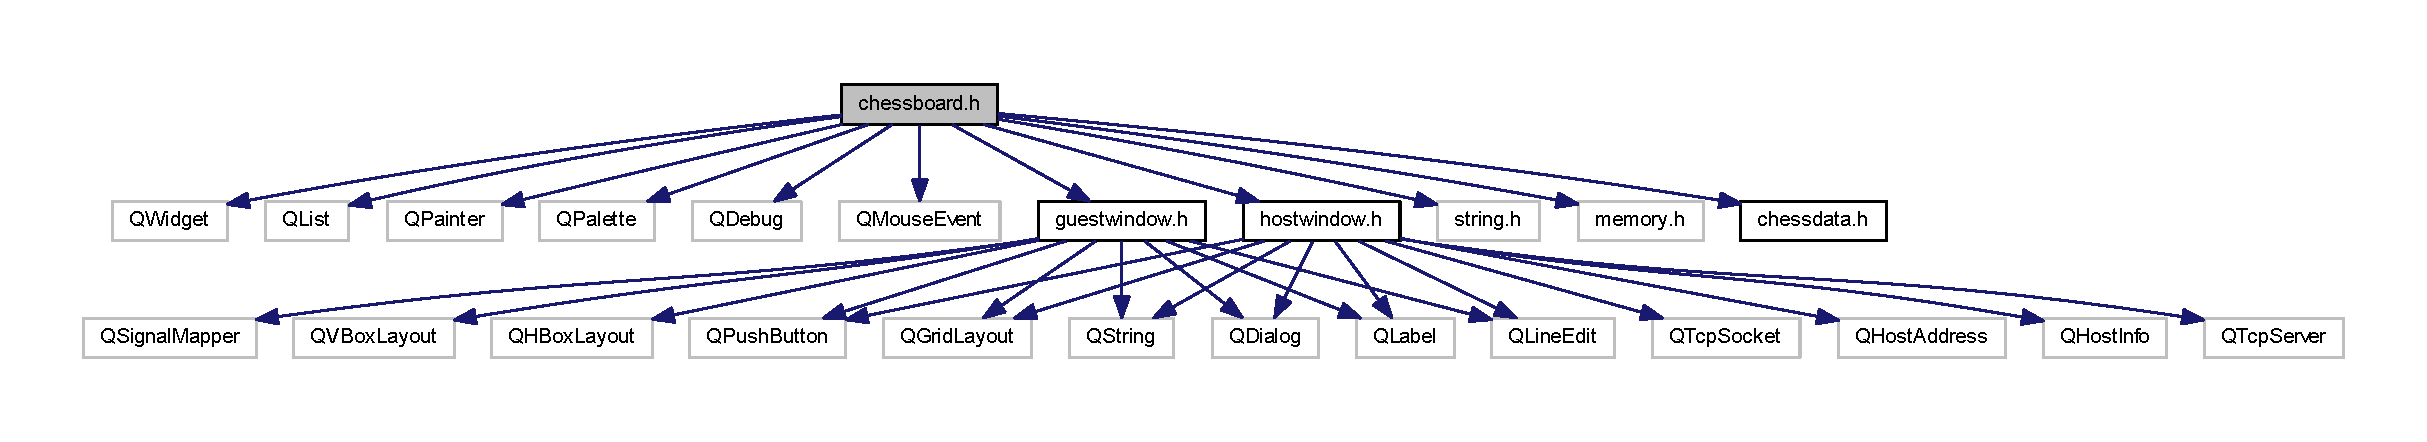
\includegraphics[width=350pt]{dd/d08/chessboard_8h__incl}
\end{center}
\end{figure}
此图展示该文件直接或间接的被哪些文件引用了\+:
\nopagebreak
\begin{figure}[H]
\begin{center}
\leavevmode
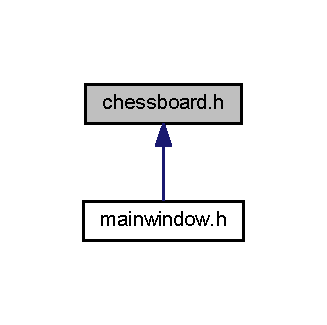
\includegraphics[width=157pt]{d0/d4f/chessboard_8h__dep__incl}
\end{center}
\end{figure}
\subsection*{类}
\begin{DoxyCompactItemize}
\item 
class \hyperlink{classchess_board}{chess\+Board}
\end{DoxyCompactItemize}

\hypertarget{chessdata_8h}{}\section{chessdata.\+h 文件参考}
\label{chessdata_8h}\index{chessdata.\+h@{chessdata.\+h}}
此图展示该文件直接或间接的被哪些文件引用了\+:
\nopagebreak
\begin{figure}[H]
\begin{center}
\leavevmode
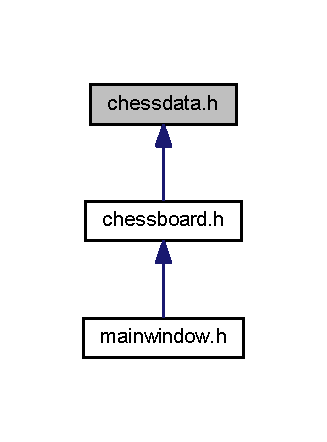
\includegraphics[width=157pt]{d2/d9d/chessdata_8h__dep__incl}
\end{center}
\end{figure}
\subsection*{类}
\begin{DoxyCompactItemize}
\item 
class \hyperlink{classchess_data}{chess\+Data}
\end{DoxyCompactItemize}

\hypertarget{guestwindow_8h}{}\section{guestwindow.\+h 文件参考}
\label{guestwindow_8h}\index{guestwindow.\+h@{guestwindow.\+h}}
{\ttfamily \#include $<$Q\+Dialog$>$}\\*
{\ttfamily \#include $<$Q\+Push\+Button$>$}\\*
{\ttfamily \#include $<$Q\+Line\+Edit$>$}\\*
{\ttfamily \#include $<$Q\+Label$>$}\\*
{\ttfamily \#include $<$Q\+Signal\+Mapper$>$}\\*
{\ttfamily \#include $<$Q\+Grid\+Layout$>$}\\*
{\ttfamily \#include $<$Q\+V\+Box\+Layout$>$}\\*
{\ttfamily \#include $<$Q\+H\+Box\+Layout$>$}\\*
{\ttfamily \#include $<$Q\+String$>$}\\*
guestwindow.\+h 的引用(Include)关系图\+:
\nopagebreak
\begin{figure}[H]
\begin{center}
\leavevmode
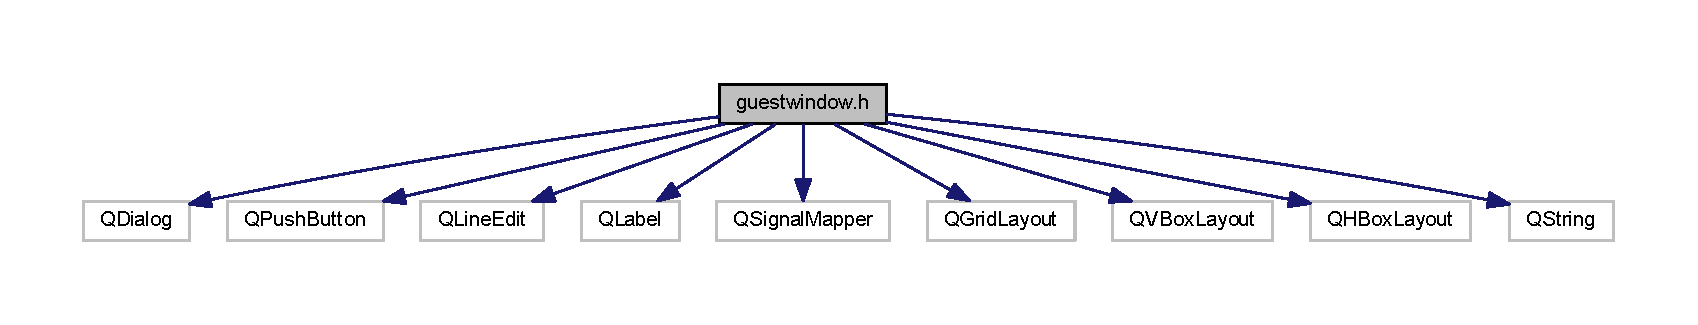
\includegraphics[width=350pt]{d8/d52/guestwindow_8h__incl}
\end{center}
\end{figure}
此图展示该文件直接或间接的被哪些文件引用了\+:
\nopagebreak
\begin{figure}[H]
\begin{center}
\leavevmode
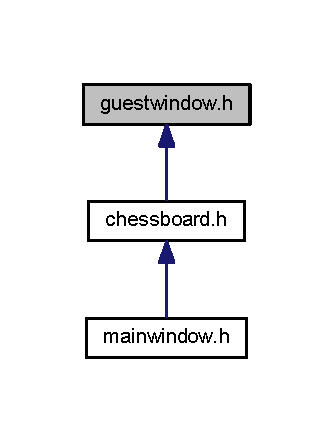
\includegraphics[width=160pt]{d6/de0/guestwindow_8h__dep__incl}
\end{center}
\end{figure}
\subsection*{类}
\begin{DoxyCompactItemize}
\item 
class \hyperlink{classguest_window}{guest\+Window}
\end{DoxyCompactItemize}

\hypertarget{hostwindow_8h}{}\section{hostwindow.\+h 文件参考}
\label{hostwindow_8h}\index{hostwindow.\+h@{hostwindow.\+h}}
{\ttfamily \#include $<$Q\+Dialog$>$}\\*
{\ttfamily \#include $<$Q\+Label$>$}\\*
{\ttfamily \#include $<$Q\+Line\+Edit$>$}\\*
{\ttfamily \#include $<$Q\+Push\+Button$>$}\\*
{\ttfamily \#include $<$Q\+Grid\+Layout$>$}\\*
{\ttfamily \#include $<$Q\+Host\+Address$>$}\\*
{\ttfamily \#include $<$Q\+Host\+Info$>$}\\*
{\ttfamily \#include $<$Q\+Tcp\+Server$>$}\\*
{\ttfamily \#include $<$Q\+Tcp\+Socket$>$}\\*
{\ttfamily \#include $<$Q\+String$>$}\\*
hostwindow.\+h 的引用(Include)关系图\+:
\nopagebreak
\begin{figure}[H]
\begin{center}
\leavevmode
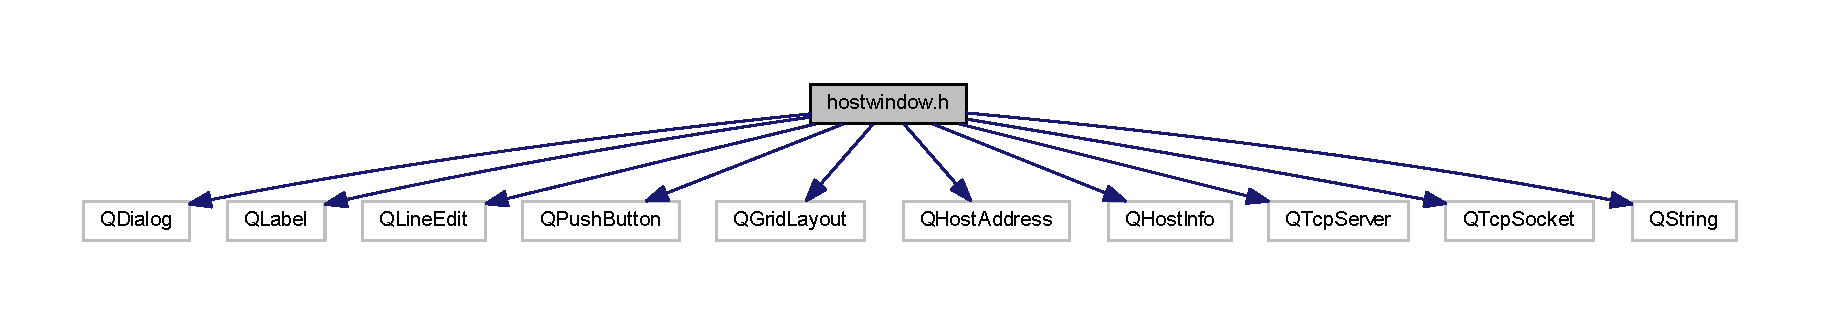
\includegraphics[width=350pt]{de/d9e/hostwindow_8h__incl}
\end{center}
\end{figure}
此图展示该文件直接或间接的被哪些文件引用了\+:
\nopagebreak
\begin{figure}[H]
\begin{center}
\leavevmode
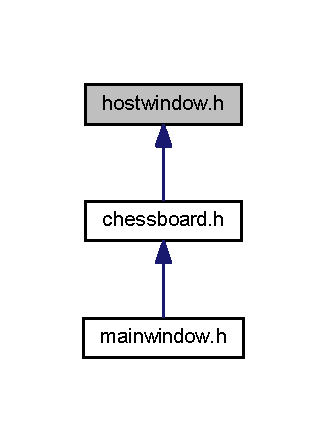
\includegraphics[width=157pt]{de/d2f/hostwindow_8h__dep__incl}
\end{center}
\end{figure}
\subsection*{类}
\begin{DoxyCompactItemize}
\item 
class \hyperlink{classhost_window}{host\+Window}
\end{DoxyCompactItemize}

\hypertarget{mainwindow_8h}{}\section{mainwindow.\+h 文件参考}
\label{mainwindow_8h}\index{mainwindow.\+h@{mainwindow.\+h}}
{\ttfamily \#include $<$Q\+Main\+Window$>$}\\*
{\ttfamily \#include $<$Q\+Tcp\+Server$>$}\\*
{\ttfamily \#include $<$Q\+Tcp\+Socket$>$}\\*
{\ttfamily \#include $<$Q\+Palette$>$}\\*
{\ttfamily \#include $<$Q\+Color$>$}\\*
{\ttfamily \#include $<$Q\+Message\+Box$>$}\\*
{\ttfamily \#include \char`\"{}chessboard.\+h\char`\"{}}\\*
mainwindow.\+h 的引用(Include)关系图\+:
\nopagebreak
\begin{figure}[H]
\begin{center}
\leavevmode
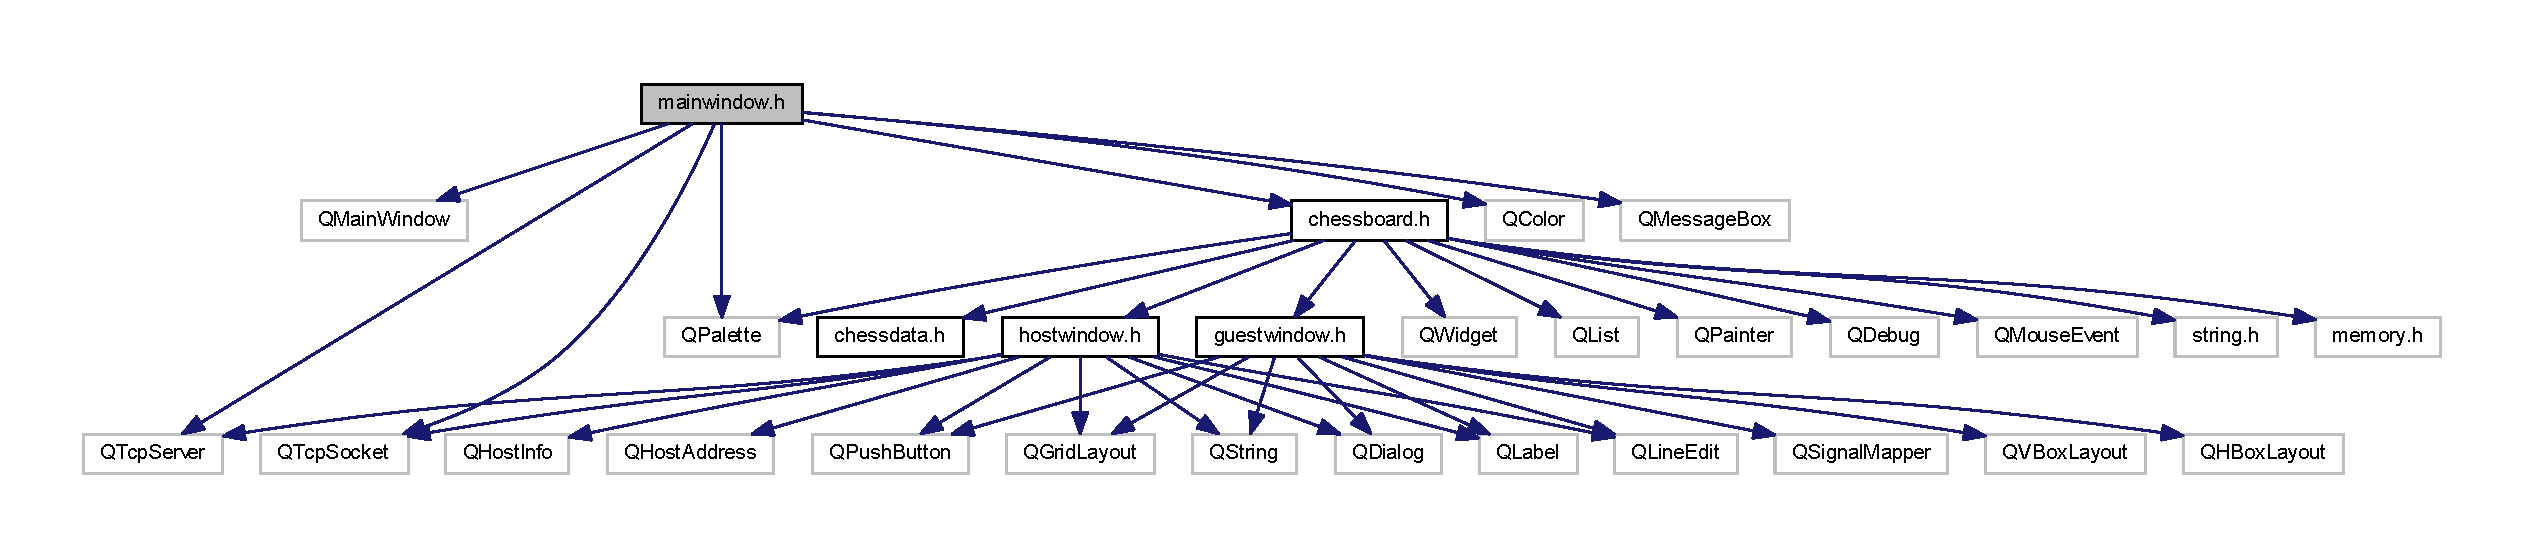
\includegraphics[width=350pt]{d2/d32/mainwindow_8h__incl}
\end{center}
\end{figure}
\subsection*{类}
\begin{DoxyCompactItemize}
\item 
class \hyperlink{class_main_window}{Main\+Window}
\end{DoxyCompactItemize}
\subsection*{命名空间}
\begin{DoxyCompactItemize}
\item 
 \hyperlink{namespace_ui}{Ui}
\end{DoxyCompactItemize}

%--- End generated contents ---

% Index
\backmatter
\newpage
\phantomsection
\clearemptydoublepage
\addcontentsline{toc}{chapter}{索引}
\printindex

\end{document}
